%latex提供的标题命令有如下九个。注意部分标题命令仅能在特定文类中使用。
    %\part
    %\chapter (report style only)
    %\section
    %\subsection
    %\subsubsection
    %\paragraph
    %\subparagraph
    %\subsubparagraph (milstd and book-form styles only)
    %\subsubsubparagraph (milstd and book-form styles only)
%标明文档使用的编码方式。UTF-8是Unicode的一种,使用它可以方便的编辑各种语言。如果没有正确设置编码方式,编译带中文的文档会产生 Package CJK Error: Invalid character code这样的错误。手动设置文档编码方式方法如下:document/document settings/format/UTF-8。使用UTF-8 + XeLaTeX排版中文文档是一种完美选择。这里我使用的是PDFTeXify或PDFLaTeX引擎,这样可以一步到位直接生成最后的PDF文件。
% !Mode:: "TeX:UTF-8"
%空行代表重启一个段落。
\chapter{IFT52\ 结合并招募\ IFT46\ 至基体}
%直接在奇数页页眉中显示章标题会多出一些章标题内部编号,这里重新定义\leftmark,后续所有章节都要重新定义
\renewcommand{\leftmark}{第五章\quad IFT52\ 结合并招募\ IFT46\ 至基体}
\section{引言}
在前一章的研究中我们鉴定到了\ IFT46\ 的基体和纤毛定位序列。同时我们发现其定位序列能够与其他\ IFT\ 蛋白相互作用形成复合物从而沿轴丝做双向运动。这暗示我们\ IFT46\ 是在其他\ IFT\ 相关蛋白的帮助下定位到基体。为了找到\ IFT46\ 的上游运载蛋白,我们拟在\ IFT\ 相关蛋白的缺失突变体中表达\ IFT46\ 或\ IFT46-C1。 如果\ IFT46\ 的基体定位不依赖某个\ IFT\ 蛋白,那么\ IFT46\ 应该能够继续定位在基体。否则,IFT46\ 将无法成功定位在基体。

\section{材料与方法}
\subsection{本研究所用仪器、试剂、培养基及溶液}
如未在正文中特别说明,本研究所用仪器、试剂、培养基及溶液信息均列于附录部分。其中,仪器信息列于
第\ \pageref{appen:A}\ 页的附录\ A,试剂信息列于第\ \pageref{appen:B}\ 页的附录\ B,培养基信息列于
第\ \pageref{appen:C}\ 页的附录\ C,溶液信息列于第\ \pageref{appen:D}\ 页的附录\ D。

\subsection{藻细胞株及菌株的培养}
本章实验所用藻株有\ CC-125\index{CC-125}、\textit{ift46-1}\index{\textit{ift46-1}}、\textit{bld1}、\textit{ift122-1}、\textit{ift88 null}、\textit{ift81-2}、\textit{dhc1b null}\ 和\ \textit{fla10-2}。其中\ \textit{ift122-1} \ 和\ \textit{ift81-2}\ 由清华大学的潘俊敏教授馈赠。通过电转化、筛选获得的藻株列于第\
\pageref{appen:E}\ 页的附录\ E。培养条件及方法
参考第\ \pageref{subsec:algae}\ 页\ \ref{subsec:algae}\ 部分。大肠埃希氏菌\index{大肠杆菌}\ DH5$\upalpha$\ 菌株由本实验室保存。培养条件及方法参考第\ \pageref{subsec:algae}\ 页\
\ref{subsec:algae}\ 部分。

\subsection{计算机辅助分析}
\textit{IFT52}\ 的基因组\ DNA\ 及蛋白序列均来源于\ Joint Genome Institute Phytozome 12\footnote{https://phytozome.jgi.doe.gov/pz/portal.html}\ 中的
\ \textit{Chlamydomonas reinhardtiiv} 5.5\ 数据库。嗜热四膜虫\ TtIFT52C/46C\ 的晶体结构文件下载自\ RCSB Protein Data Bank\footnote{http://www.rcsb.org/pdb/home/home.do}(ID:4UZZ)
\citep{Taschner2014}。衣藻\ CrIFT52C/46C\ 的三维结构根据\ TtIFT52C/46C\ 的晶体结构利用\ Phyre2\ 进行模拟产生\ \citep{Kelley2015}。获得的结构文件用\ Protein Workshop
\citep{Moreland2005,Xu2009}\ 进行观察并找出\ IFT52C\ 和\ IFT46C\ 结合界面上关键的疏水残基用于定点突变。

\subsection{分子克隆}
如未作特殊说明,分子克隆所用方法参考第\ \pageref{subsec:melcular cloning}\ 页\
\ref{subsec:melcular cloning}\ 部分和第\ \pageref{subsec:melcular cloning second}\ 页
\ \ref{subsec:melcular cloning second}\ 部分。

%开始图片浮动体环境,其中!表示取消严谨限制,h表示在此处插入,t表示在本页或下一页顶部插入
\begin{figure}[!ht]
%居中对齐
\centering
%设置图片搜索路径,每个路径用{}括起来
\graphicspath{{figures/}}
%插入图片并设置图片宽度为文本宽度减10mm

\includegraphics[width=\textwidth-30mm]{fig5-1.jpg}
%生成中英双语标题
{\setstretch{1.667}
\bicaption[fig:5.1]{图}{In-Fusion\ 同源重组克隆方法示意图。通过\ PCR\ 获得的\ DNA\ 片段和线性化载体被\ In-Fusion\ 重组酶融合成完整载体。图中彩色方框代表重叠的\ 15 bp\ 片段。}{Figure}{Schematic diagram of In-Fusion HD cloning method. PCR-generated sequences and linearized vector are fused together by In-Fusion enzyme. Colored boxes at ends of DNA fragments are 15 bp overlap.}
\par}
%结束图片浮动体环境
\end{figure}

\subsubsection{In-Fusion\ 同源重组克隆}\label{subsubsec:in fusion}
In-Fusion\ 同源重组克隆的原理如图\ \ref{fig:5.1}\ 所示\ \citep{Marsischky2004,Gibson2009}。使用\ In-Fusion HD Cloning Kit (Clontech, Cat\#639636),按表\
\ref{tab:table5.1}\ 加入各试剂后混匀,瞬时离心后\ \SI{50}{\degreeCelsius}\ 反应三十分钟,冰上静置一分钟。将所有的反应产物用于热激转化,转化方法参考第\ \pageref{subsub:heat transformation}\ 页\ \ref{subsub:heat transformation}\ 部分。从平板上挑二十四个单克隆至含有\ \SI{1}{\mL}\ LB\ 液体培养基(含\ \SI{100}{\ug}/\si{\mL}\ 氨苄青霉素)的\ \SI{2}{\mL}\ 离心管中,\SI{37}{\degreeCelsius}\ 培养过夜后进行菌液\ PCR\ 鉴定,引物为\ IFT52seq-F\ 和\ IFT52seq-R。选择三个阳性克隆扩大培养抽提质粒进行酶切验证。

%开始表格浮动体环境,其中!表示取消严谨限制,h表示在此处插入,t表示在本页或下一页顶部插入
\begin{table}[!ht]
%居中对齐
\centering
%生成中英双语标题
{\setstretch{1.667}
\bicaption[tab:table5.1]{表}{In-Fusion\ 同源重组克隆反应体系}{Table}{Reaction system for In-Fusion cloning}
\par}
%更改表格内文字的字号
\small
%开始绘制表格
\begin{tabular*}{\textwidth}[c]{@{\extracolsep{\fill}}lll}
%绘制一条水平线
\toprule
编号\ (Number) & 试剂\ (Reagents)       & 质量或体积\ (Mass or Volume)\\
\midrule
1 & IFT52 promoter                              & \SI{100}{\ng}\\
2 & IFT52C                                      & \SI{100}{\ng}\\
3 & \textit{Nde}I \textit{Sda}I digested pHK470 & \SI{50}{\ng}\\
4 & 5x In-Fusion Enzyme Premix                  & \SI{1}{\uL}\\
5 & ddH$_2$O                                    & To \SI{5}{\uL}\\
\bottomrule
%结束绘制表格
\end{tabular*}
%结束表格浮动体环境
\end{table}

\subsubsection{定点突变}\label{subsubsec:SDM}
使用全式金点突变试剂盒进行定点突变,基本原理如图\
\ref{fig:5.2}\ 所示\
\citep{Higuchi1988,Zheng2004,Ko2005}。具体步骤如下。

(1)使用\ GeneTool Lite\ 设计引物\ SDM-F\ 和\ SDM-R。

(2)使用下列体系进行\ PCR\ 扩增:质粒模板,5 ng;\SI{10}{\micro\nauticalmile}\ SDM-F,1 $\upmu$L;10 $\upmu$M SDM-R,1 $\upmu$L;2xTransStart FastPfu PCR SuperMix,25 $\upmu$L;ddH$_2$O,至\ 50 $\upmu$L。其中质粒模板必须来源于非甲基化缺陷型菌株,如实验室常用的\ DH5$\upalpha$\ 和\ DH10$\upbeta$。PCR \ 反应程序如下:
\SI{95}{\degreeCelsius}\ 预变性五分钟;\SI{95}{\degreeCelsius},二十秒;\SI{60}{\degreeCelsius},二十秒;
\SI{72}{\degreeCelsius},两分钟;循环二十次;\SI{72}{\degreeCelsius}\ 补时延伸十分钟。

(3)向\ PCR\ 产物中加入\ \SI{1}{\uL} DMT\ 酶,混匀后瞬时离心,\SI{37}{\degreeCelsius}\ 孵育一小时。

(4)取\ \SI{5}{\uL} DMT\ 酶消化产物加入到\ \SI{50}{\uL}\ 感受态细胞中进行热激转化,具体步骤参考
第\ \pageref{subsub:heat transformation}\ 页\ \ref{subsub:heat transformation}\ 部分。

(5)取\ \SI{200}{\uL}\ 菌液均匀的涂在抗性平板上,在\ \SI{37}{\degreeCelsius}\ 培养箱中过夜培养。

(6)挑取单克隆接种到含\ 1 mL LB\ 培养基(含\ 100 $\upmu$g/mL\ 的氨苄青霉素)的\ \SI{1.5}{\mL}\ 离心管中培养过夜,取\ \SI{100}{\uL}\ 菌液测序。选择突变成功的单克隆抽提质粒进行后续实验。

%开始图片浮动体环境,其中!表示取消严谨限制,h表示在此处插入,t表示在本页或下一页顶部插入
\begin{figure}[!ht]
%居中对齐
\centering
%设置图片搜索路径,每个路径用{}括起来
\graphicspath{{figures/}}
%插入图片并设置图片宽度为文本宽度减10mm
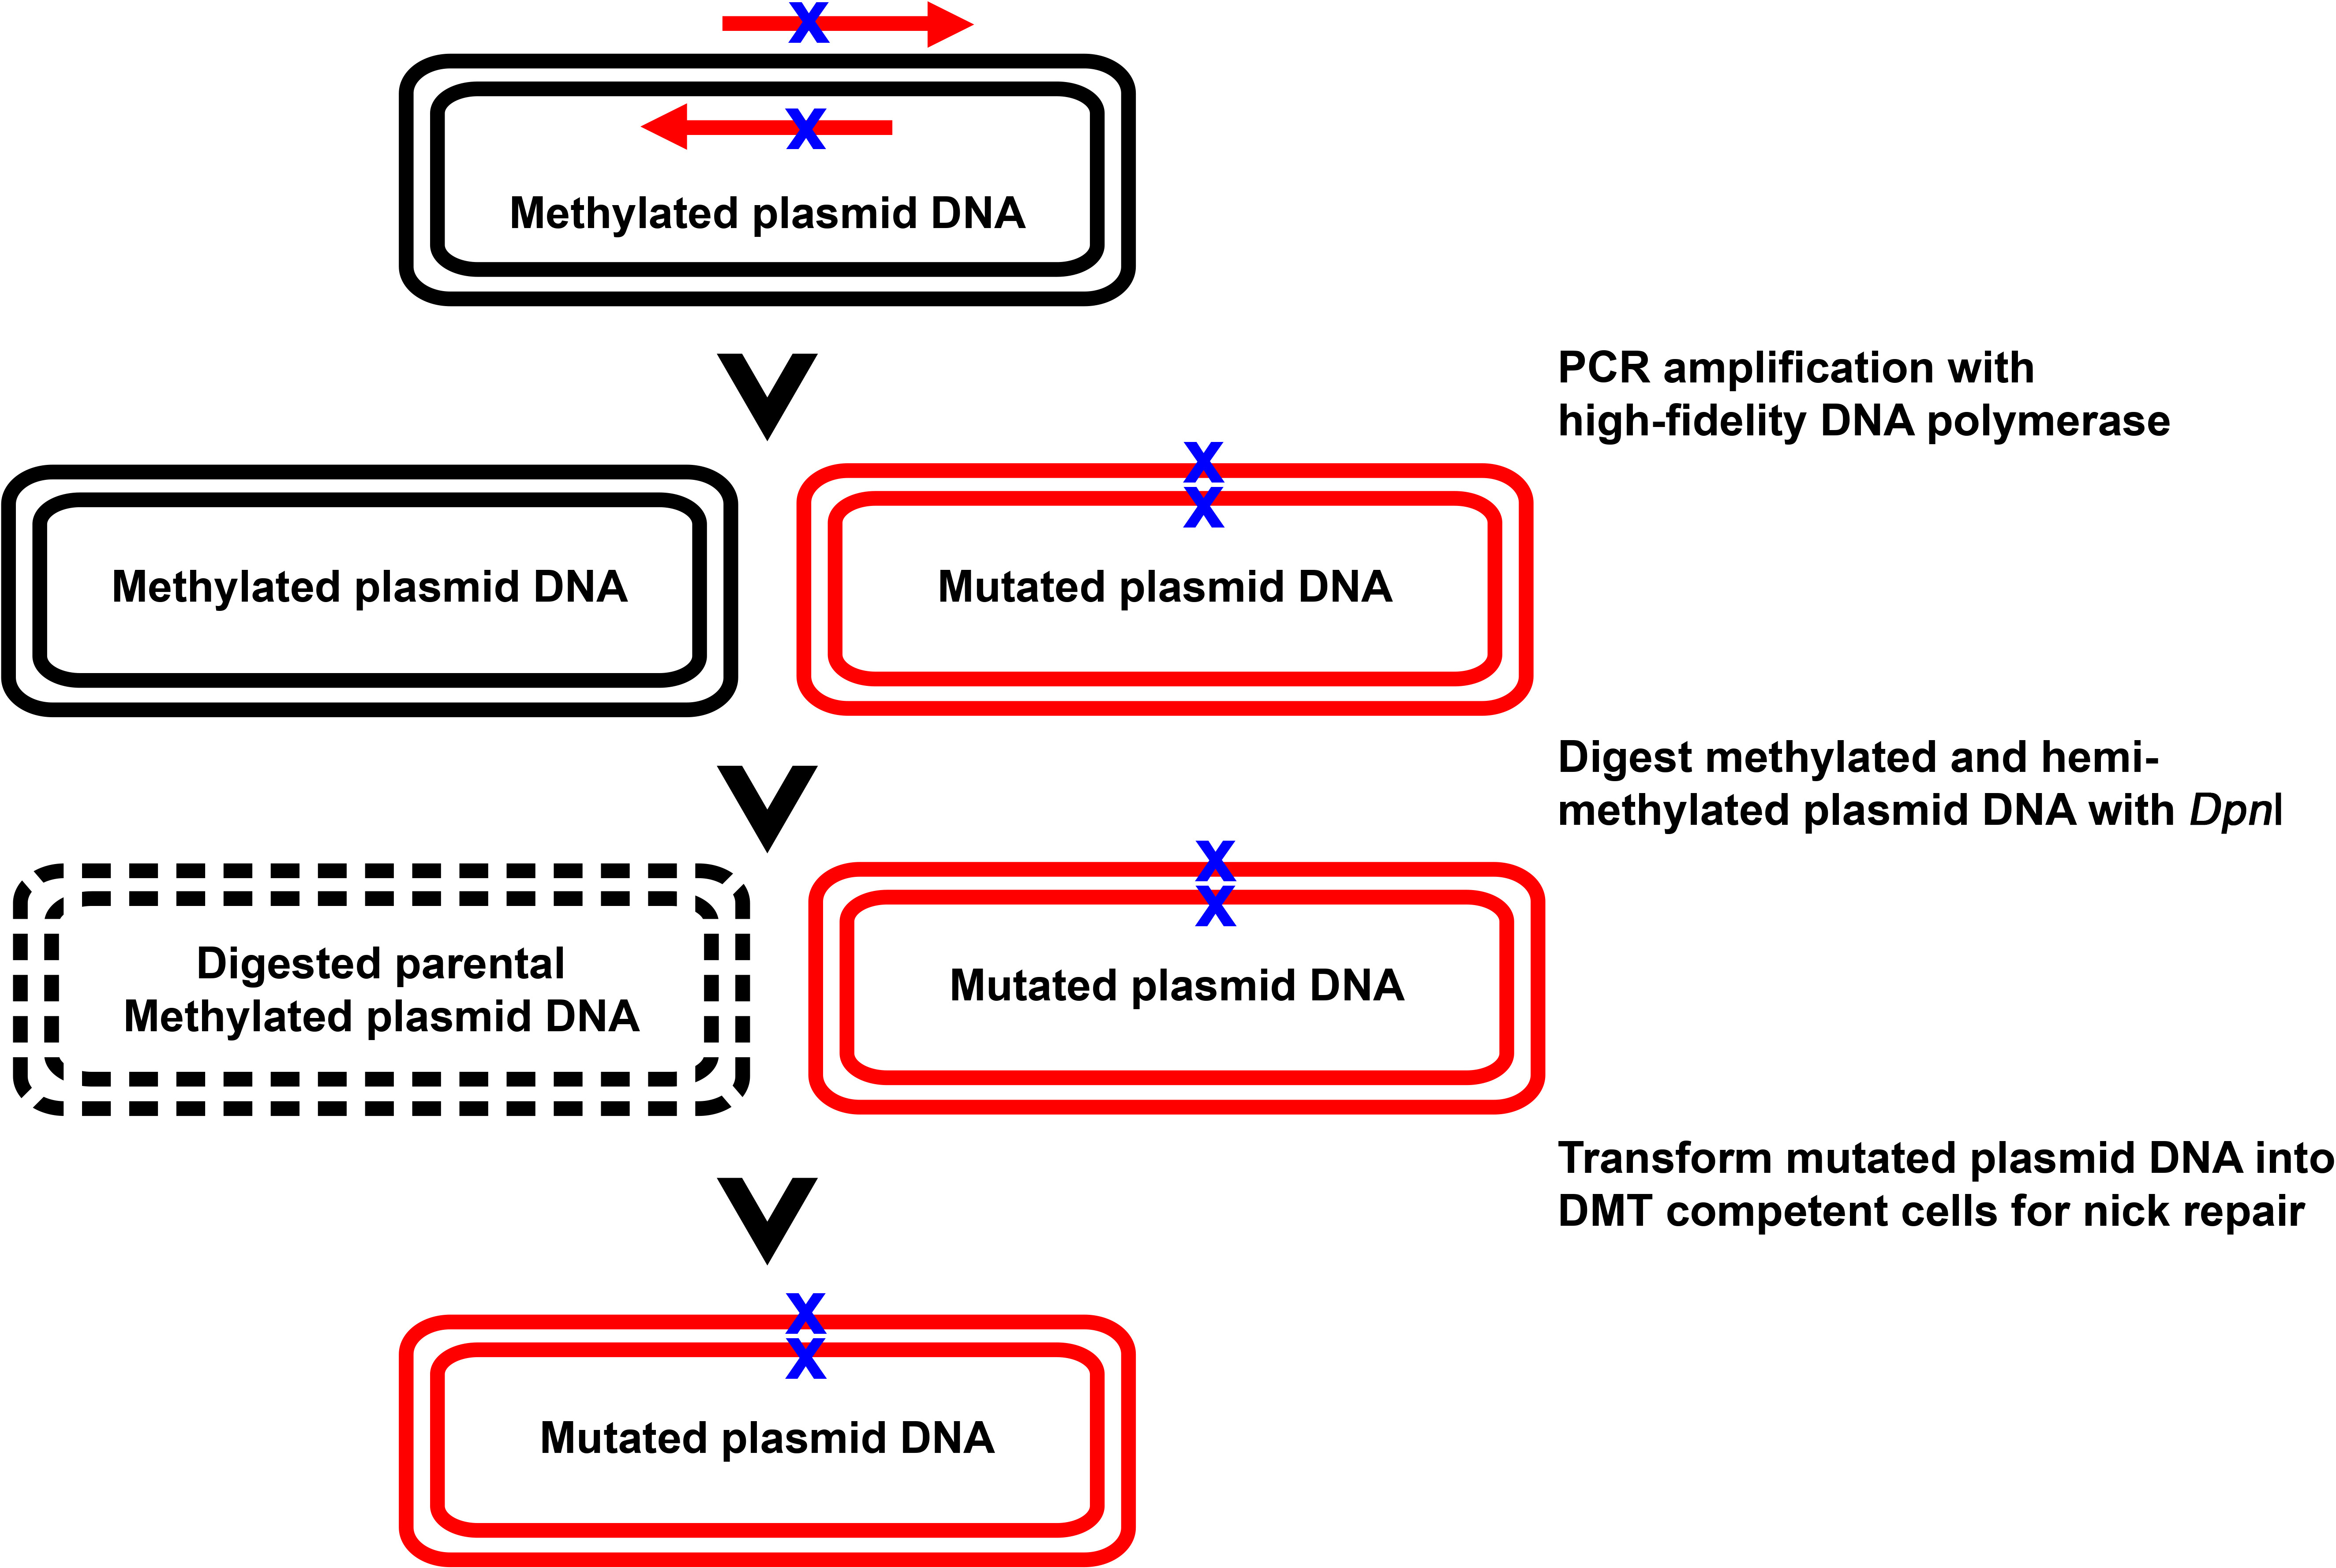
\includegraphics[width=\textwidth]{fig5-2.jpg}
%生成中英双语标题
{\setstretch{1.667}
\bicaption[fig:5.2]{图}{定点突变原理示意图。首先利用重叠引物通过反向\ PCR\ 扩增获得带突变的质粒。然后用\
\textit{Dpn}I\ 消化甲基化和半甲基化的模板。最后将消化后的产物转化至\ DMT\ 感受态细胞中完成缺口修复。} {Figure}{Overview of the TRANS Fast Site-directed Mutagenesis System. The first step is to obtain mutated plasmid DNA using overlapped primers through reverse PCR. Then, the methylated and semi-methylated plasmid DNA in the amplification products are digested with \textit{Dpn}I. Finally, digested-products are transformed into DMT competent cells for nick repair.}
\par}
%结束图片浮动体环境
\end{figure}

\subsubsection{载体构建}
为了拯救\ \textit{IFT52}\ 的缺失突变体\ \textit{bld1},我们构建了\ pHK250(表达\ IFT52::YFP\ 和巴龙霉素抗性基因)、pHK268 (表达\ IFT52::YFP\ 和潮霉素抗性基因)和\ pHK409(表达\ IFT52::3HA\ 和巴龙霉素抗性基因)。
以\ CC-503\ 的基因组\ DNA\ 为模板,用引物\ IFT52A-F\ 和\ IFT52B-R\ 扩增\ \textit{IFT52}\ 的基因组\ DNA。 扩增产物经\
\textit{Nde}I/\textit{Eco}RV\ 双酶切后连接到\ \textit{Nde}I/\textit{Eco}RV\ 消化后的\ pHK86\ 或\ pHK266,分别获得\ pHK250\ 和\ pHK268。为了在\ IFT52\ 的\ C\ 端融合\ 3xHA\ 标签,使用寡核苷酸\ HA1、HA2、HA3\ 和\ HA4\ 退火合成\ 3xHA\ 的核酸序列并连接到\ \textit{Eco}RV/\textit{Eco}RI\ 消化后的\ pHK250,由此获得表达\ IFT52::3HA\ 的\ pHK409\
(参考第\ \pageref{subsec:oligoanneal}\ 页\ \ref{subsec:oligoanneal}\ 部分)。

使用\ \textit{Nde}I/\textit{Eco}RV\ 将\ IFT46-C1\ 的编码序列从\ pHK245\ 上切割下来并将其连接到\ \textit{Nde}I/\textit{Eco}RV\ 消化后的\ pHK266\ 中,由此获得表达\ IFT46-C1\ 和潮霉素抗性基因的\ pHK242。 为了破坏\ IFT46-C1\ 和\ IFT52\ 之间的相互作用,我们使用引物\ SDM-F\ 和\ SDM-R\ 对\ pHK242\ 进行了定点突变
(参考第\ \pageref{subsubsec:SDM}\ 页\ \ref{subsubsec:SDM}\ 部分)。由此产生的载体\ pHK267\ 可表达\ IFT46-C1$^{L285E/L286E}$::YFP。

为了构建表达\ YFP::NLS\ 的\ pHK464,我们利用\ \textit{Eco}RV/\textit{Eco}RI\ 双酶切将\ pHK469\ 上的第二个\ \textit{yfp}\ 基因切除并插入\ 4xSV40 NLS。4xSV40 NLS\ 是通过五条寡核苷酸\ 4xNLS-1F、4xNLS-2R、4xNLS-3F、4xNLS-4R\ 和\ 4xNLS-5R\ 退火产生的。以\ pHK464\ 为模板,用引物\ NLS-F\ 和\ NLS-R\ 扩增\ \textit{yfp}-NLS\ 序列。扩增产物经\
\textit{Sma}I/\textit{Eco}RI\ 双酶切后连接到经\ \textit{Eco}RV/\textit{Eco}RI\ 消化后的\ pHK409 \ 中,由此获得\ pHK470。为了构建表达\ IFT52C::YFP::NLS\ 的\ pHK473,我们以\ pHK470\ 为模板,利用引物\ IFT52C-F\ 和\ IFT52C-R\ 进行扩增,扩增产物经纯化后利用\ In-Fusion\ 方法重组克隆(参考第\ \pageref{subsubsec:in fusion}\ 页\ \ref{subsubsec:in fusion}\ 部分)。

\subsubsection{质粒提取}
使用\ Omega\ 去内毒素质粒小提试剂盒进行质粒提取,具体步骤如下。

(1)取\ 1-\SI{5}{\mL}\ 细菌培养物,室温\ \SI{12000}{\g}\ 离心一分钟,尽量吸除上清。

(2)向留有菌体沉淀的离心管中加入\ \SI{250}{\uL}\ Solution I\ (请先检查是否已加入\ RnaseA),使用移液器或涡旋振荡器彻底悬浮细菌细胞沉淀。

(3)向离心管中加入\ \SI{250}{\uL}\ Solution II,温和地上下翻转四至六次使菌体充分裂解。注意混匀一定要温和,以免污染细菌基因\ DNA,此时菌液应变得清亮粘稠,作用时间不要超过五分钟,以免质粒受到破坏。但也不要低于两分钟,以免裂解不充分。

(4)向离心管中加入\ \SI{125}{\uL}\ 冰冷的\ Buffer N3,立即温和地上下翻转六至八次,充分混匀,此时会出现白色絮状沉淀。最大转速室温离心十分钟,用移液器小心地将上清转移到另一个干净的离心管中,尽量不要吸出沉淀。

(5)加入上清十分之一体积\ ETR Solution,温和的颠倒七至十次混匀,将离心管置于冰上静置十分钟,期间颠倒离心管数次。

 (6)\SI{42}{\degreeCelsius}\ 水浴五分钟,不时振荡,溶液又变浑浊。\SI{12000}{\g}\ 室温离心三分钟,溶液应分为两相,上层水相含质粒\ DNA,下层蓝色油状相含内毒素。

(7)将含质粒\ DNA\ 的上层水相转移至\ \SI{2}{\mL}\ 离心管中,加入二分之一体积的无水乙醇。温和的上下颠倒六至十次,室温静置两分钟。

(8)将(7)中的液体通过离心收集到\ HiBind\ 柱子中。

(9)加入\ \SI{500}{\uL}\ Buffer HB,\SI{12000}{\g}\ 离心一分钟,倒掉收集管中的废液。

(10)向吸附柱中加入\ \SI{700}{\uL}\ DNA Wash Buffer(使用前请先检查是否已加入无水乙醇),\SI{12000}{\g}\ 离心一分钟,弃废液,将吸附柱放入收集管中。

(11)重复步骤(10)一次。

 (11)\SI{12000}{\g}\ 离心三分钟,将吸附柱敞口置于室温或\ \SI{50}{\degreeCelsius}\ 温箱放置数分钟,目的是将吸附柱中残余的漂洗液去除,否则漂洗液中的乙醇会影响后续的实验如酶切、PCR\ 等。

 (12)将吸附柱放入一个干净的离心管中,向吸附膜中央悬空滴加\ 80-\SI{100}{\uL}\ 经\ \SI{65}{\degreeCelsius}\ 水浴预热的无内毒素洗脱液,室温放置两分钟,\SI{12000}{\g}\ 离心一分钟。

\subsection{衣藻电转化}
参考第\ \pageref{subsec:electrotransformation}\ 页\ \ref{subsec:electrotransformation}\ 部分。

\subsection{autolysin\ 的制备}\label{subsec:autolysin}
参考\ \textit{Chlamydomonas} Resource Center\footnote{http://www.chlamycollection.org/}上提供的关于\ autolysin\ 制备的方法(Preparation of Gamete Autolysin\footnote{http://www.chlamycollection.org/methods/preparation-of-gamete-autolysin/})并稍作修改,具体步骤如下。

(1)将\ CC-125(mt+)和{} CC-124(mt-)分别从\ TAP\ 平板上转接至含\ \SI{150}{\mL}{} TAP\ 培养基的三角瓶内,震荡培养至细胞浓度约\ \num{3.0e6}{} cells/\si{\mL}。

(2)将上一步活化的细胞分别转移至含有\ \SI{500}{\mL}{} TAP\ 培养基的三角瓶内,震荡培养至细胞浓度约\ \num{3.0e6}{} cells/\si{\mL}。

(3)\SI{1500}{\g}\ 离心五分钟,弃上清。沉淀用\ \SI{500}{\mL}{} M-N\ 培养基重悬后再次离心弃上清。用\ \SI{1}{\L}{} M-N\ 培养基重悬后分装至两个\ \SI{2}{\L}\ 的三角瓶中,此时藻细胞浓度应接近
\ \num{1.0e6}{} cells/\si{\mL}。

(4)连续光照震荡培养\ 18-19\ 小时诱导配子形成。后期定时取\ \SI{700}{\uL}\ 不同交配型的细胞,混匀后离心并用\ \SI{70}{\uL}{} M-N\ 重悬,三十分钟后镜检观察交配情况。

(5)若交配效率大于百分之八十则\ \SI{20}{\degreeCelsius},\SI{1600}{\g}\ 离心五分钟收集细胞,细胞沉淀用\ \SI{50}{\mL}{} M-N\ 重悬,此时细胞密度约\ \num{4.0e7}{} cells/\si{\mL}。

(6)震荡培养六十分钟左右使鞭毛恢复。若鞭毛率高于百分之五十则可进行交配。

(7)将等量不同交配型的配子细胞混合后强光低速震荡孵育三十分钟。交配过程中配子细胞会释放\ autolysin。

(8)\SI{20}{\degreeCelsius},\SI{3500}{\g}\ 离心七分钟,将上清转移到\ \SI{50}{\mL}\ 离心管中,
\ \SI{9000}{\g}\ 离心十五分钟,取上清用\ \SI{0.45}{\um}\ 滤器过滤除菌并于
\ \SI{-20}{\degreeCelsius}\ 保存备用。

\subsection{衣藻细胞核提取}
使用植物叶片细胞核提取试剂盒并参考\ \citet{Winck2011}\ 的方法进行衣藻细胞核提取,具体步骤如下。

(1)培养\ \SI{250}{\mL}\ 藻细胞至对数早期(细胞浓度约\ \num{6.0d6}\  cells/mL),\SI{4}{\degreeCelsius},3500 g\ 离心两分钟收集藻细胞。用\ \SI{50}{\mL}{} autolysin\ 处理细胞六十分钟后离心回收\ autolysin,沉淀用\ 5 mL 1xNIB\ 溶液洗涤一次。再次离心弃上清,沉淀用\ \SI{600}{\uL}\  1xNIB\ 溶液重悬。衣藻\ autolysin\ 的制备方法参考第\ \pageref{subsec:autolysin}\ 页\
\ref{subsec:autolysin}\ 部分。

(2)将悬液转移到用液氮预冷的研钵中研磨成黄\textcolor{green}{绿色}粉末。

(3)将粉末转移到\ 50 mL\ 圆底离心管中,加入\ 10 mL 1xNIBA\ 溶液,混匀后冰上静置十分钟。

(4)使用水平转头离心机\ \SI{4}{\degreeCelsius},1260 g\ 离心十分钟,弃上清。

(5)用\ 10 mL\ 含\ 1\%\ Triton X-100\ 的\ 1xNIBA\ 重悬沉淀,用移液管吹打混匀后瞬时离心,冰上静置十分钟。使用水平转头离心机\ \SI{4}{\degreeCelsius},1000 g\ 离心三十分钟,弃上清。

(6)取沉淀重复裂解一次,离心弃上清。

(7)用\ 1 mL 1xNIBA重悬沉淀并转移到\ 2 mL离心管中,\SI{4}{\degreeCelsius},600 g\ 离心十分钟,弃上清。重复洗涤一次即得到乳白色细胞核沉淀。

(8)用\ \SI{50}{\uL}\ 保存液重悬沉淀并置于\ \SI{-80}{\degreeCelsius}\ 保存。

\subsection{SDS-PAGE\ 及免疫印迹分析}
SDS-PAGE\ 参考第\ \pageref{subsec:SDS-PAGE}\ 页\ \ref{subsec:SDS-PAGE}\ 部分。免疫印迹分析
参考第\ \pageref{subsec:western}\ 页\ \ref{subsec:western}\ 部分。检测所用抗体的信息见第\
\pageref{appen:H}\ 页的附录\ H。

\subsection{衣藻免疫荧光}
衣藻的免疫荧光参考已有方法\ \citep{Wykoff1999,Wood2012,Kusnier2006,LeDizet1986,Deane2001}\ 并稍作修改,具体步骤如下。检测所用抗体的信息见第\ \pageref{appen:H}\ 页的附录\ H。

(1)将盖玻片置于无水乙醇中浸泡过夜,取出后室温晾干并置于\ 0.1\%\ 聚乙烯亚胺\footnote{Polyethyleneimine, PEI} 中浸泡两分钟,室温晾干备用。

(2)取\ 1 mL\ 处于对数生长期的藻细胞(细胞密度约\ \num{4.0d6} cells/mL),3000 g\ 室温离心一分钟,弃上清。

(3)沉淀用\ \SI{1}{\mL}\ 新鲜\ TAP\ 培养基重悬,室温静置两分钟后离心弃上清。

(4)沉淀用\ \SI{100}{\uL} PBS\ 缓冲液重悬后备用。

(5)取\ \SI{50}{\uL}\ 藻液滴加在盖玻片中央,室温静置十分钟使藻细胞沉降吸附在盖玻片上。

(6)将盖玻片置于\ \SI{-20}{\degreeCelsius}\ 甲醇中浸泡十分钟后室温晾干五分钟,用\ PBS\ 缓冲液浸泡三次,每次五分钟。

(7)向盖玻片中央滴加\ \SI{200}{\uL}\ 山羊血清封闭液室温封闭一小时。

(8)移除封闭液,使用含有一抗的山羊血清封闭液\ \SI{4}{\degreeCelsius}\ 孵育过夜。

(9)移除一抗孵育液,使用含\ 0.5\%\ 吐温\ 20\ 的\ PBS\ 缓冲液洗涤三次,每次十分钟。

(10)使用含有二抗的山羊血清封闭液室温孵育一小时。

(11)移除二抗孵育液,使用含\ 0.5\%\ 吐温\ 20\ 的\ PBS\ 缓冲液洗涤三次,每次十分钟。最后用去离子水洗涤一次后彻底移除盖玻片上的液体。加\ \SI{5}{\uL}\ 抗荧光淬灭剂后将盖玻片覆盖在载玻片上并移除气泡。使用无色指甲油封闭四周。

(12)将制备的玻片置于暗盒中干燥两小时以上。若不立即进行显微观察可置于\ \SI{4}{\degreeCelsius}\ 长期保存。

\subsection{免疫共沉淀}
免疫共沉淀参考第\ \pageref{subsec:CoIP}\ 页\ \ref{subsec:CoIP}\ 部分。

\subsection{GST pull-down\ 分析}
本实验由德国马普生化所的\ Esben Lorentzen\ 教授(现为丹麦奥胡斯大学分子生物与遗传系
副教授\footnote{www.mbg.au.dk/en/research/research-areas/structural-biology/esben-lorentzen/})实验室完成,以下为简要的实验步骤。

(1)将\ CrIFT46(包括野生型和突变型)和\ CrIFT52C\ 单独或同时转化至大肠杆菌\ BL21(DE3)\ 感受态细胞中。

(2)挑取单克隆在\ LB\ 液体培养基中培养至\ OD600\ 为\ 1,此过程中保持培养温度为\
\SI{37}{\degreeCelsius}。

(3)将培养温度调整到\ \SI{18}{\degreeCelsius},向培养基中加入终浓度为\ 0.5 mM\ 的\ IPTG\ 诱导蛋白表达。维持该条件培养过夜。

(4)取\ 100 $\upmu$L\ 培养液室温\ 25000 g\ 离心\ 3\ 分钟,沉淀用\ 50 $\upmu$L\ 的\ 1xSDS\ 上样缓冲液重悬后沸水煮十分钟。裂解液室温\ 25000 g\ 离心十分钟,上清即为大肠杆菌全细胞裂解液。

(5)将其余的细胞沉淀用裂解液重悬,细胞悬液于\ \SI{4}{\degreeCelsius} 25000 g\ 离心三十分钟,收集上清用于\ GST pull-down\ 分析。

(6)取上步中的上清与\ GSH-resin\ 于\ \SI{4}{\degreeCelsius}\ 孵育两小时,用裂解液洗涤珠子两次,然后用含\ 20 mM\ 还原型谷胱甘肽的裂解液将珠子上结合的蛋白洗脱下来。

(7)将大肠杆菌裂解液及\ GST pull-down\ 分析实验中的洗脱液用\ SDS-PAGE\ 进行分析。

\subsection{显微观察}
显微观察及活细胞成像参考第\ \pageref{subsec:microscope}\ 页\ \ref{subsec:microscope}\ 部分。

\subsection{统计分析}
参考第\ \pageref{subsec:statistics}\ 页\ref{subsec:statistics}\ 部分。

\section{结果}
%开始图片浮动体环境,其中!表示取消严谨限制,h表示在此处插入,t表示在本页或下一页顶部插入
\begin{figure}[h!tbp]
%居中对齐
\centering
%设置图片搜索路径,每个路径用{}括起来
\graphicspath{{figures/}}
%插入图片并设置图片宽度为文本宽度减10mm
\includegraphics[width=\textwidth]{fig5-3.jpg}
%生成中英双语标题
{\setstretch{1.45}
\bicaption[fig:5.3]{图}{IFT46\ 的基体定位不依赖\ IFT122, IFT88, IFT81, FLA10\ 或\ DHC1b。(A,B,D,E,G,H)全细胞裂解物免疫印迹分析。(C,F,I)藻株的共聚焦成像分析。白色箭头标示眼点。(J,K)藻株\ \textit{ift81-2}\ (J)和\ \textit{ift122-1}\ (K)的免疫荧光成像。
\textcolor{red}{红色}为乙酰化\ $\upalpha$-tubulin,\textcolor{green}{绿色}为\ IFT46,\textcolor{blue}{蓝色}为标示细胞核的\ DAPI。 在\ A、B、D、E、G\ 和\ H\ 中,每个泳道的上样量为\ \SI{5}{\ug}。CHL\ 代表叶绿色。IB\ 代表免疫印迹。在\ C、F、I、J\ 和\ K\ 中,标尺代表\ \SI{5}{\um}.}{Figure}{The basal body localization of IFT46 is independent of IFT122, IFT88, IFT81, FLA10 or DHC1b. (A, B, D, E, G, H) Western blots of whole-cell lysates of indicated strains. (C, F, I) Confocal imaging of indicated strains. White arrows mark the eyespots. (J, K) Immunofluorescence microscopy of \textit{ift81-2} (J) and ift122-1 (K) using anti-acetylated $\upalpha$-tubulin antibody (red), anti-IFT46 antibody (green) and DAPI (blue). In A, B, D, E, G, and H, five micrograms of protein were loaded into each lane. IB means immunoblot. In C, F, I, J, and K, scale bars represent 5 $\upmu$m. CHL means chlorophyll.}
\par}
%结束图片浮动体环境
\end{figure}

\subsection{IFT46\ 的基体定位不依赖\ IFT122、IFT88、IFT81、FLA10\ 或\ DHC1b}
根据已发表的结果,我们知道\ IFT46\ 至少与\ ODA16、IFT88、IFT81、IFT74、IFT70\ 和\ IFT52\ 存在相互作用\
\citep{Lucker2005,Lucker2010,Taschner2014,Taschner2011,Fan2010}。我们的问题是\ IFT46\ 的基体定位是否依赖其他\ IFT\ 组分。为解决这一问题,我们拟在\ IFT\ 相关的缺失突变体中表达\ IFT46::YFP\ 或\ IFT46-C1::YFP。 如果\ IFT46\ 的基体定位依赖某个组分,那么\ IFT46::YFP\ 或\ IFT46-C1::YFP\ 将无法继续定位在基体。

据此,我们在\ \textit{ift88}、\textit{fla10-2}\ 和\ \textit{dhc1b}\ 中表达了\ IFT46::YFP\ 或\ IFT46-C1::YFP
(图\ \ref{fig:5.3}A,B,D,E,G,H)。 这些藻株分别是\ IFT88、FLA10\ 和\ DHC1b\ 的缺失突变体。使用抗\ GFP\ 的抗体通过免疫印迹我们筛选到了阳性克隆(图
\ref{fig:5.3}A,B,D,E,G,H)。同时我们也通过免疫荧光观察了\ IFT46\ 在\ \textit{ift81-2}\ 和\ \textit{ift122-1}\ 中的亚细胞定位(图\ \ref{fig:5.3}J,K)。观察结果显示,IFT46::YFP\ 或\ IFT46-C1::YFP\ 仍然定位在\
\textit{ift88}、\textit{fla10-2}\ 或\ \textit{dhc1b}\ 的基体(图\ \ref{fig:5.3}C,F,I)。这表明\ IFT46\ 的基体定位不依赖\ IFT88、FLA10\ 或\ DHC1b。 在\ \textit{ift81-2}\ 或\ \textit{ift122-1} 中,IFT46\ 与乙酰化\ $\upalpha$\ 微管蛋白共定位,后者主要定位在突变体的基体和短小鞭毛中(图\ \ref{fig:5.3}J,K)。这些结果意味着\ IFT46\ 的基体定位在\ \textit{ift81-2}\ 或\
\textit{ift122-1}\ 中并未受到影响,其基体定位也不依赖\ IFT81\ 或\ IFT122。

\subsection{IFT46\ 的基体定位依赖\ IFT52}
%开始图片浮动体环境,其中!表示取消严谨限制,h表示在此处插入,t表示在本页或下一页顶部插入
\begin{figure}[h!tbp]
%居中对齐
\centering
%设置图片搜索路径,每个路径用{}括起来
\graphicspath{{figures/}}
%插入图片并设置图片宽度为文本宽度减10mm
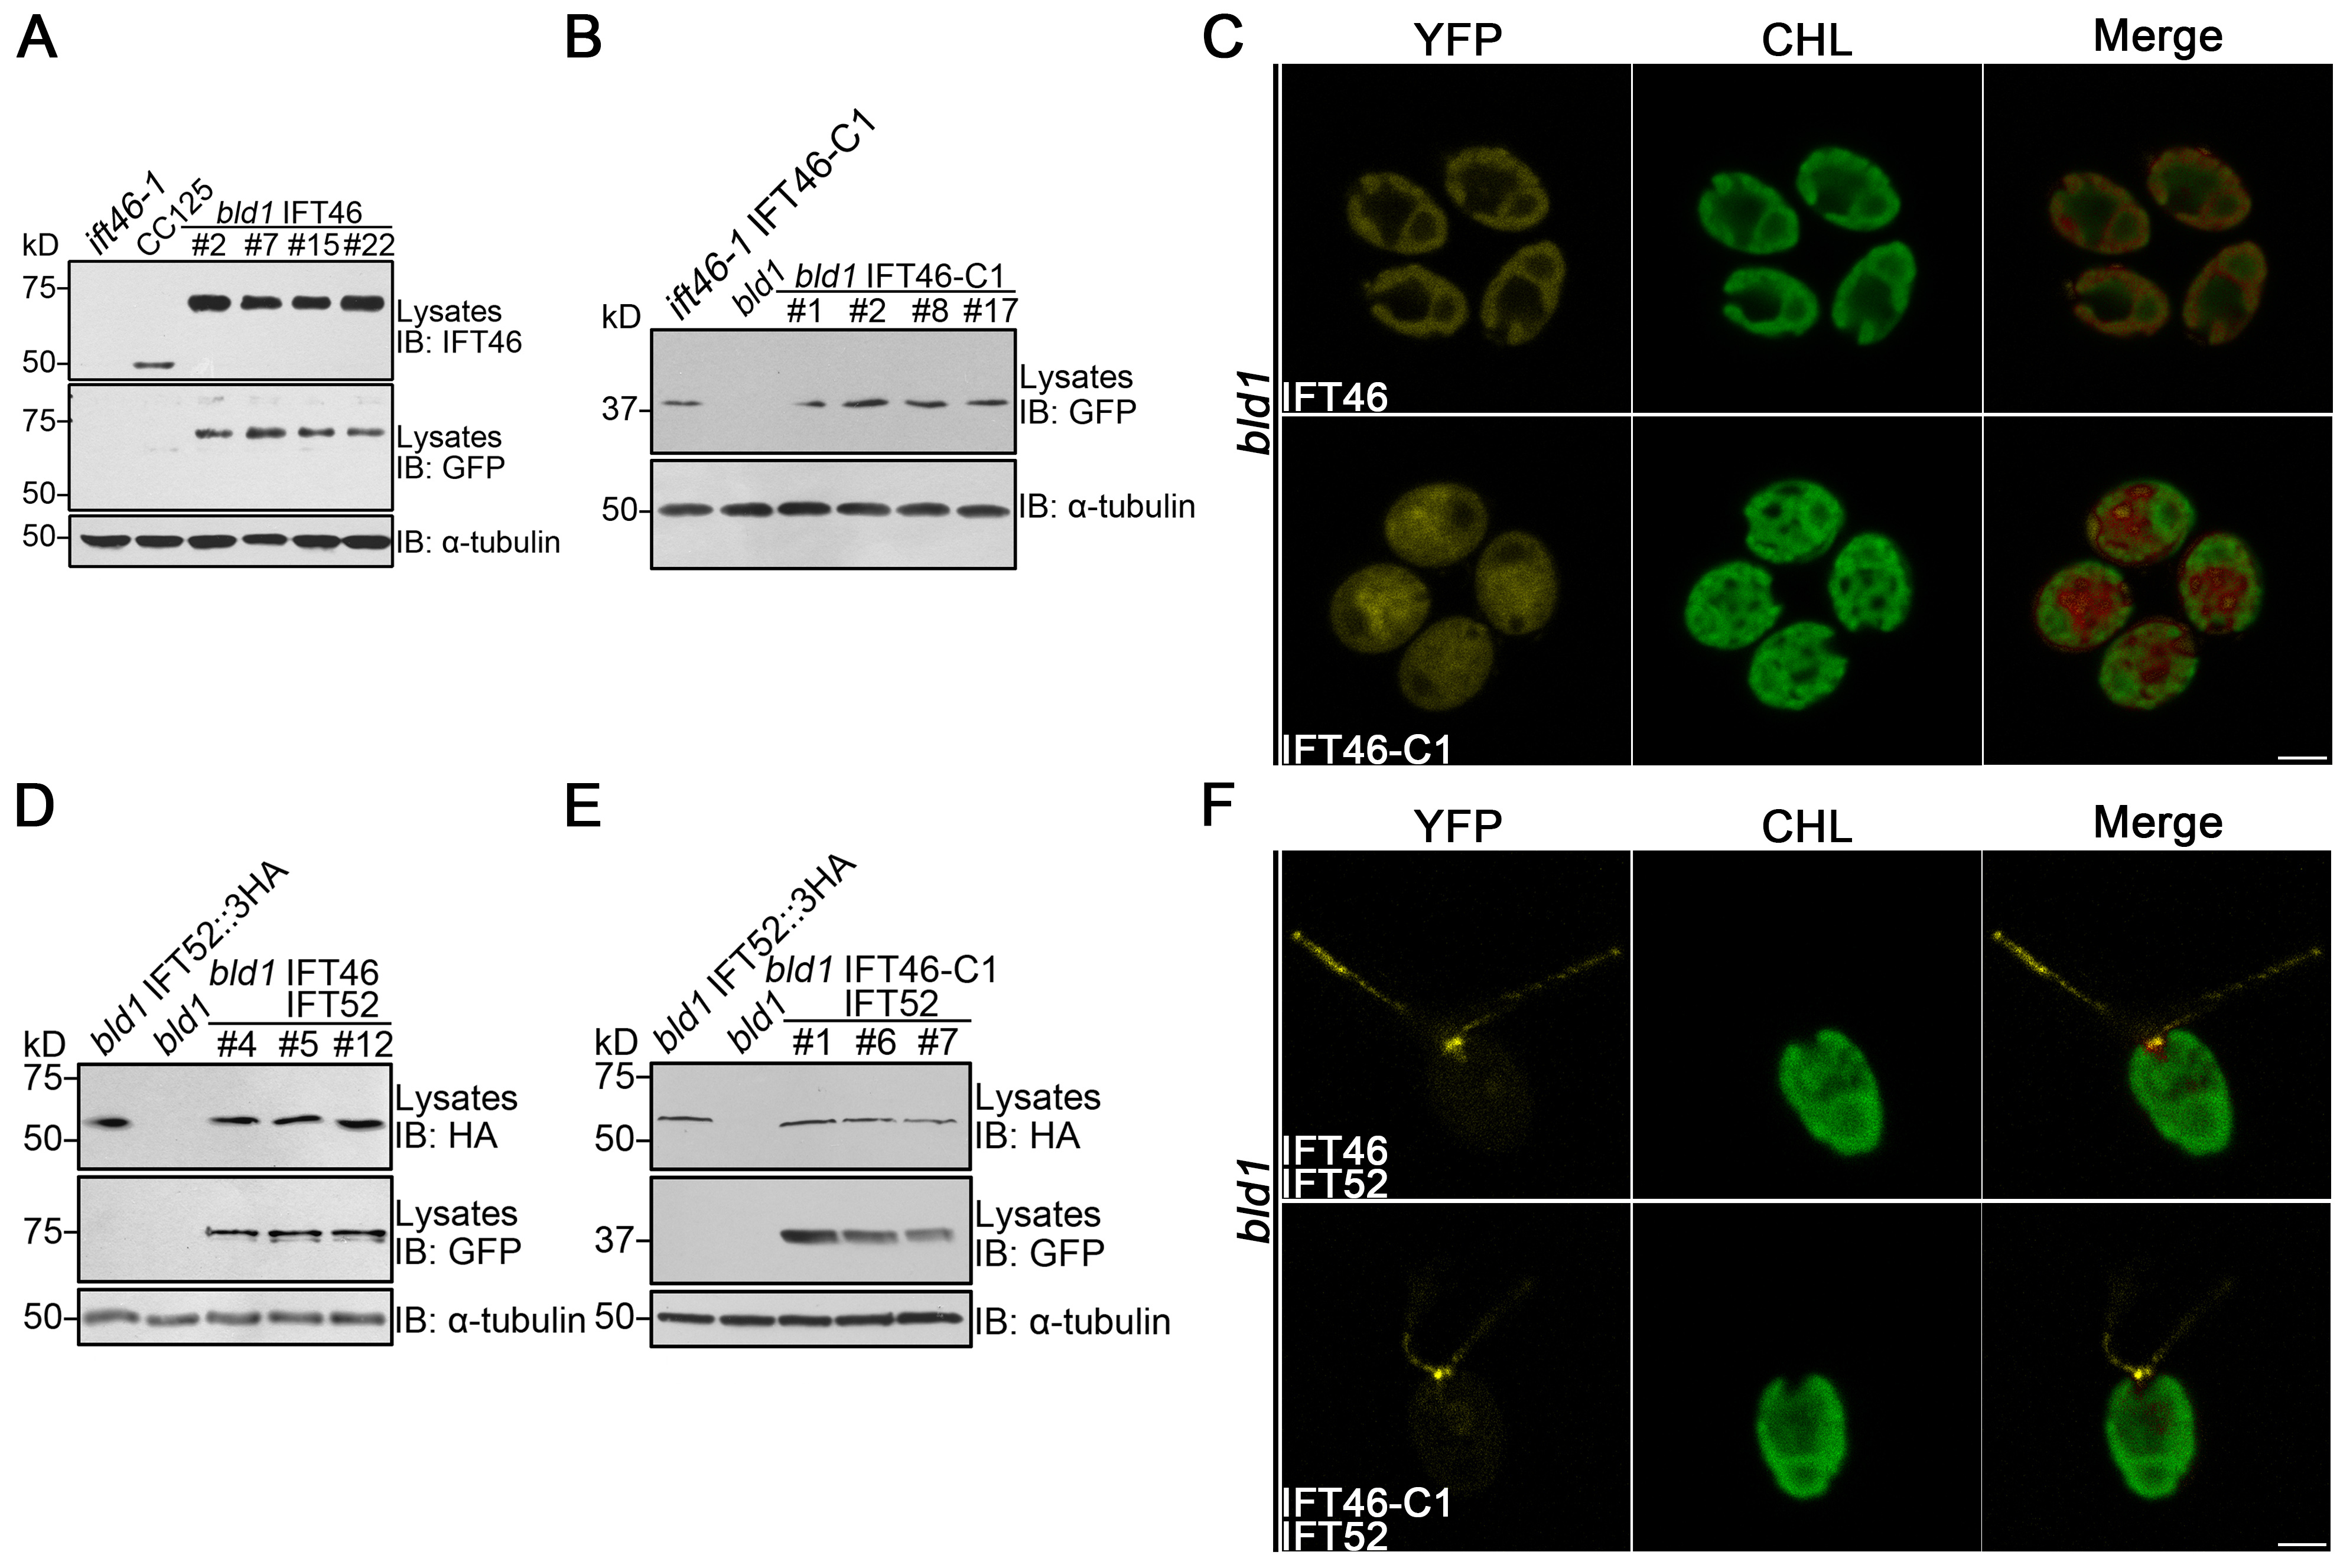
\includegraphics[width=\textwidth]{fig5-4.jpg}
%生成中英双语标题
{\setstretch{1.55}
\bicaption[fig:5.4]{图}{IFT46\ 的基体定位依赖\ IFT52。(A) \textit{bld1}, CC-125\ 和
\textit{bld1} \textit{IFT46::YFP}\ 全细胞裂解物免疫印迹分析。IB\ 代表免疫印迹。(B) \textit{ift46-1} \textit{IFT46-C1::YFP}, \textit{bld1}\ 和\ \textit{bld1} \textit{IFT46-C1::YFP}\ 全细胞裂解物免疫印迹分析。IB\ 代表免疫印迹。(C)表达\ IFT46::YFP\ 或\ IFT46-C1::YFP\ 的\ \textit{bld1}\ 藻株的共聚焦成像分析。(D)\textit{bld1} \textit{IFT52::3HA}, \textit{bld1}\ 和\ \textit{bld1} \textit{IFT46::YFP IFT52::3HA}\ 全细胞裂解物免疫印迹分析。IB\ 代表免疫印迹。(E)\textit{bld1} \textit{IFT52::3HA}, \textit{bld1}\ 和\ \textit{bld1} \textit{IFT46-C1::YFP IFT52::3HA}\ 全细胞裂解物免疫印迹分析。IB\ 代表免疫印迹。(F)表达\ IFT46::YFP IFT52::3HA\ 或\ IFT46-C1::YFP IFT52::3HA\ 的\ \textit{bld1}\ 藻株的共聚焦成像分析。在\ C\ 和\ F\ 中标尺代表\ \SI{5}{\um}。}{Figure}{The basal body localization of IFT46 depends on IFT52. (A) Western blots of whole-cell lysates of \textit{bld1}, CC-125, and \textit{bld1} \textit{IFT46::YFP} probed with the anti-GFP antibody and anti-$\upalpha$-tubulin antibody. IB: immunoblot. (B) Western blots of whole-cell lysates of \textit{ift46-1} \textit{IFT46-C1::YFP}, \textit{bld1}, and \textit{bld1} \textit{IFT46-C1::YFP} probed with the indicated antibodies. IB: immunoblot. (C) Confocal imaging of \textit{bld1} expressing IFT46::YFP or IFT46-C1::YFP. (D) Western blots of whole-cell lysates of \textit{bld1} \textit{IFT52::3HA}, \textit{bld1}, and \textit{bld1} \textit{IFT46::YFP IFT52::3HA} probed with the indicated antibodies. IB: immunoblot. (E) Western blots of whole-cell lysates of \textit{bld1} \textit{IFT52::3HA}, \textit{bld1}, and \textit{bld1} \textit{IFT46-C1::YFP IFT52::3HA} probed with the indicated antibodies.IB: immunoblot. (F) Confocal imaging of \textit{bld1} expressing IFT46::YFP IFT52::3HA or IFT46-C1::YFP IFT52::3HA. In panel C and F, CHL means chlorophyll. Scale bars represent 5 $\upmu$m.}
\par}
%结束图片浮动体环境
\end{figure}

同样的,我们也在\ \textit{IFT52}\ 的缺失突变体\ \textit{bld1}\ 中表达了\ IFT46\ 或\ IFT46-C1 (图
\ref{fig:5.4}\allowbreak A,B)。对阳性克隆的观察结果显示\ IFT46\ 无法继续定位在\ \textit{bld1} \ 的基体周围(图
\ref{fig:5.4}C)。IFT52\ 处于\ IFT-B\ 复合物的核心,它与\ IFT-B1\ 和\ IFT-B2\ 的多个亚基之间均存在相互作用\
\citep{Taschner2016a,Lucker2005,Lucker2010,Taschner2011,Taschner2014,Katoh2016}。IFT52\ 的缺失可导致\ IFT-B\ 其他亚基的表达量下降\ \citep{Zhang2016,Deane2001,Collet1998,Brazelton2001}。然而,\ IFT46\ 或\ IFT46-C1\ 无法定位在\
\textit{bld1}\ 的基体不太可能是由表达量下降造成的。因为我们观察的阳性克隆是通过免疫印迹筛选到的高表达株(图\ \ref{fig:5.4}A,B)。总之,IFT46\ 的基体定位依赖\ IFT52。

如果\ IFT52\ 的缺失能够破坏\ IFT46\ 的基体定位,那么理论上重新表达\ IFT52\ 应该能够恢复\ IFT46\ 的基体定位。为了验证这一点,我们在\ \textit{bld1} \textit{IFT46::YFP}\ 或\ \textit{bld1} \textit{IFT46-C1::YFP} 中表达了\ IFT52::3HA (图
\ref{fig:5.4}C,D)。通过对筛选到的阳性克隆进行共聚焦成像,我们发现在\ \textit{bld1} \textit{IFT46::YFP IFT52::3HA}\ 或\ \textit{bld1} \textit{IFT46-C1::YFP IFT52::3HA}\ 中\ IFT46\ 又重新定位到了基体(图
\ref{fig:5.4}E)。这些结果进一步说明\ IFT46\ 的基体定位确实依赖\ IFT52。

然而,IFT46\ 的基体定位依赖\ IFT52\ 还是存在两种可能性。一种是二者的依赖是相互的,它们共同作用从而靶向基体。另一种是\ IFT52\ 作用在\ IFT46\ 的上游,IFT52\ 将\ IFT46\ 招募到基体。为了排除其中一种可能性,我们在\ \textit{IFT46}\ 的缺失突变体\
\textit{ift46-1}\ 中表达了\ IFT52::YFP(图
\ref{fig:5.5}A)。使用抗\ GFP\ 的抗体通过免疫印迹我们筛选到了阳性克隆。活细胞成像结果显示\ IFT52\ 能够正常定位到\
\textit{ift46-1}\ 的基体(图\ \ref{fig:5.5}B)。这表明\ IFT52\ 的基体定位并不依赖\ IFT46,IFT52\ 作用在\ IFT46\ 的上游。

%开始图片浮动体环境,其中!表示取消严谨限制,h表示在此处插入,t表示在本页或下一页顶部插入
\begin{figure}[ht]
%居中对齐
\centering
%设置图片搜索路径,每个路径用{}括起来
\graphicspath{{figures/}}
%插入图片并设置图片宽度为文本宽度减10mm
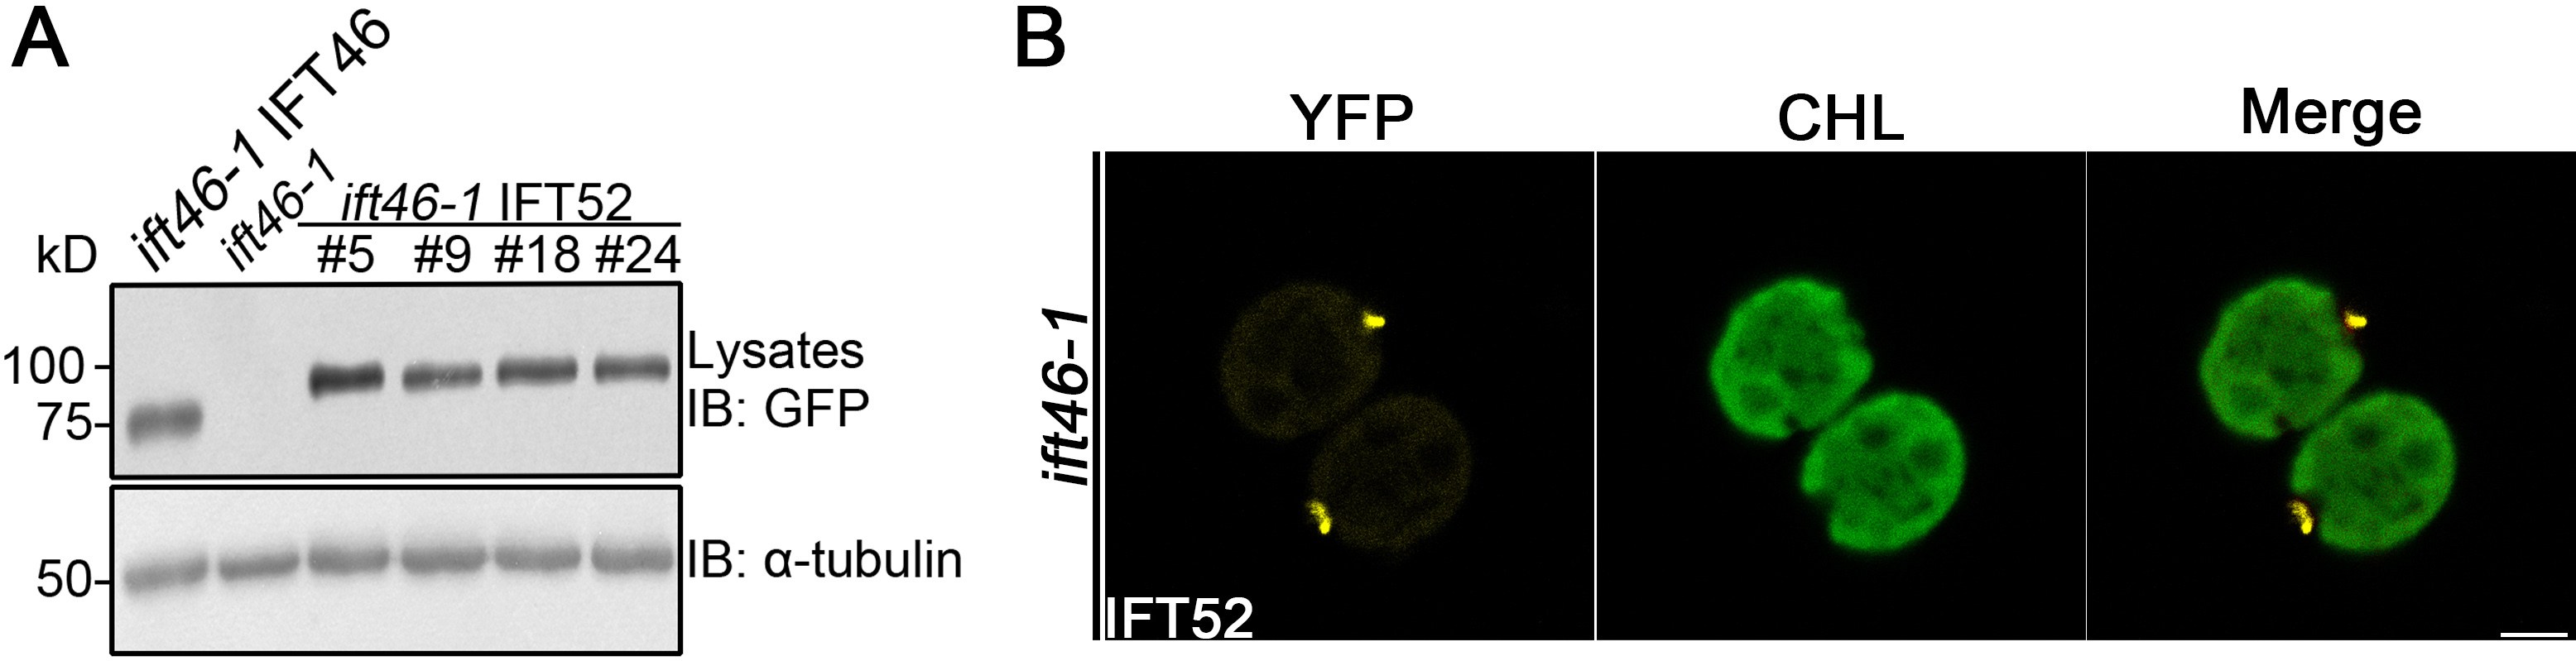
\includegraphics[width=\textwidth]{fig5-5.jpg}
%生成中英双语标题
{\setstretch{1.667}
\bicaption[fig:5.5]{图}{IFT52\ 的基体定位不依赖\ IFT46。(A)\textit{ift46-1} \textit{IFT46::YFP}, \textit{ift46-1}\ 和\ \textit{ift46-1} \textit{IFT52::YFP}\ 全细胞裂解物免疫印迹分析。每个泳道的上样量为\ \SI{5}{\ug}。IB\ 代表免疫印迹。(B)表达\ IFT52::YFP\ 的
\ \textit{ift46-1}\ 藻株的共聚焦成像分析。标尺代表\ \SI{5}{\um}。}{Figure}{The basal body localization of IFT52 does not depend on IFT46. (A) Western blots of whole-cell lysates of \textit{ift46-1} \textit{IFT46::YFP}, \textit{ift46-1}, and \textit{ift46-1} \textit{IFT52::YFP} probed with the indicated antibodies. Five micrograms of protein were loaded per lane. IB means immunoblot. (B) Confocal imaging of \textit{ift46-1} expressing IFT52::YFP. CHL means chlorophyll. Scale bar represents 5 $\upmu$m.}
\par}
%结束图片浮动体环境
\end{figure}

\subsection{IFT52\ 结合并招募\ IFT46\ 至基体}
IFT52\ 和\ IFT46\ 之间的相互作用已经在体外实验中得到验证\
\citep{Taschner2016a,Lucker2005,Lucker2010,Taschner2011,Taschner2014,Katoh2016}。这里我们发现\ IFT46\ 的基体定位依赖\ IFT52。因而我们猜测二者之间的相互作用可能介导了\ IFT46\ 的基体定位。使用抗\ HA\ 的抗体对\ \textit{bld1} \textit{IFT46-C1::YFP IFT52::3HA}\ 的全细胞裂解液进行免疫共沉淀分析,结果显示\ IFT46\ 或\ IFT46-C1\ 富集在沉淀物中(图
\ref{fig:5.6}A)。这表明\ IFT46-C1\ 与全长\ IFT46\ 一样也能够与\ IFT52\ 相互作用。

%开始图片浮动体环境,其中!表示取消严谨限制,h表示在此处插入,t表示在本页或下一页顶部插入
\begin{figure}[h!btp]
%居中对齐
\centering
%设置图片搜索路径,每个路径用{}括起来
\graphicspath{{figures/}}
%插入图片并设置图片宽度为文本宽度减10mm
\includegraphics[width=\textwidth]{fig5-6.jpg}
%生成中英双语标题
{\setstretch{1.4}
\bicaption[fig:5.6]{图}{IFT52\ 结合并招募\ IFT46\ 至基体。(A)\ 用抗\ HA\ 的抗体对\ CC-125, \textit{bld1} \textit{IFT52::3HA}\ 和\ \textit{bld1} \textit{IFT46-C1 IFT52::3HA}\ 全细胞裂解液进行免疫共沉淀分析。(B)\ IFT46\ 定点突变示意图。(C)\ 基于\ TtIFT52C/46C\ 模拟的\ CrIFT52C/46C\ 的晶体结构。(D)\ Pull-down\ 分析显示\ GST-IFT52C\ 与\ IFT46$^{WT}$\ 相互作用,但不与\ IFT46$^{L285E/L286E}$\ 相互作用。(E)\ 全细胞裂解物免疫印迹分析。(F)\ IFT46-C1$^{L285E/L286E}$\ 相对于\ IFT46-C1\ 表达量显著下降。(G)\ 藻株的共聚焦成像分析。白色箭头表示眼点。CHL\ 代表叶绿素。标尺代表\ \SI{10}{\um}。}{Figure}{IFT52 binds and recruits IFT46 to the basal body. (A) Anti-HA antibody was used to immunoprecipitate HA-tagged IFT52. (B) Schematic diagram of site-directed mutagenesis of \textit{IFT46} gene. (C) The crystal structure of CrIFT52C/46C modeled based on TtIFT52C/46C. The two residues for mutagenesis were highlighted as grey sticks. (D) Pull-down of His-tagged GST-IFT52(366-454) with untagged IFT46$^{WT}$ or IFT46$^{L285E/L286E}$. (E) Western blots of whole-cell lysates (\SI{3}{\ug} protein per lane) of indicated strains. (F) Relative expression level of IFT46-C1$^{L285E/L286E}$ compared to the expression level of IFT46-C1. (G) Confocal imaging of indicated strains. White arrows, eyespots; CHL, chlorophyll; Scale bar, 10 $\upmu$m.}
\par}
%结束图片浮动体环境
\end{figure}

为了进一步测试\ IFT52\ 与\ IFT46\ 之间的相互作用是否是\ IFT46\ 基体定位所必须的,我们将\ IFT46-C1\ 上的两个关键的疏水亮氨酸突变为谷氨酸(图\ \ref{fig:5.6}B)。这两个亮氨酸在进化上高度保守(图\ \ref{fig:4.10})。从\ CrIFT52C/46C\ 的晶体结构(依据\ TtIFT52C/46C\ 的晶体结构模拟产生)上可以看到二者位于\ IFT52C\ 和\ IFT46C\ 的结合界面上
(图\ \ref{fig:5.6}C)\citep{Taschner2014}。将\ IFT52C\ 与突变后的\ IFT46\ 共表达在大肠杆菌中,结果显示\ IFT46$^{L285E/L286E}$\ 无法继续结合\ IFT52C(图\ \ref{fig:5.6}D)。与野生型\ IFT46-C1\ 相比,表达在\ \textit{ift46-1}\ 中的\ IFT46-C1$^{L285E/L286E}$\ 的表达量下降至约\ 32\%(
图\ \ref{fig:5.6}E,F)。由于\ IFT46$^{L285E/L286E}$\ 无法与\ IFT52\ 相互作用形成复合物,这种表达量的下降很可能是由于游离的\ IFT46-C1$^{L285E/L286E}$\ 被降解造成的。如图\ \ref{fig:5.6}G\ 所示,IFT46-C1\ 中第\ 285\ 和\ 286\ 号残基的突变破坏了其基体定位。由于\ IFT46-C1\ 和\ BBTS3\ 在表达量下降至约\ 30\%\ 时仍然能够定位到基体(图\ \ref{fig:4.9},\ref{fig:4.8}),IFT46-C1$^{L285E/L286E}$\ 的基体定位消失应该不是由于表达量下降造成的。这些结果表明\ IFT46-C1\ 与\ IFT52\ 之间的相互作用对\ IFT46\ 的基体定位至关重要。IFT52\ 结合并招募\ IFT46\ 至基体。

\subsection{构建表达\ IFT52C::YFP::NLS\ 的载体}
%开始图片浮动体环境,其中!表示取消严谨限制,h表示在此处插入,t表示在本页或下一页顶部插入
\begin{figure}[ht]
%居中对齐
\centering
%设置图片搜索路径,每个路径用{}括起来
\graphicspath{{figures/}}
%插入图片并设置图片宽度为文本宽度减10mm
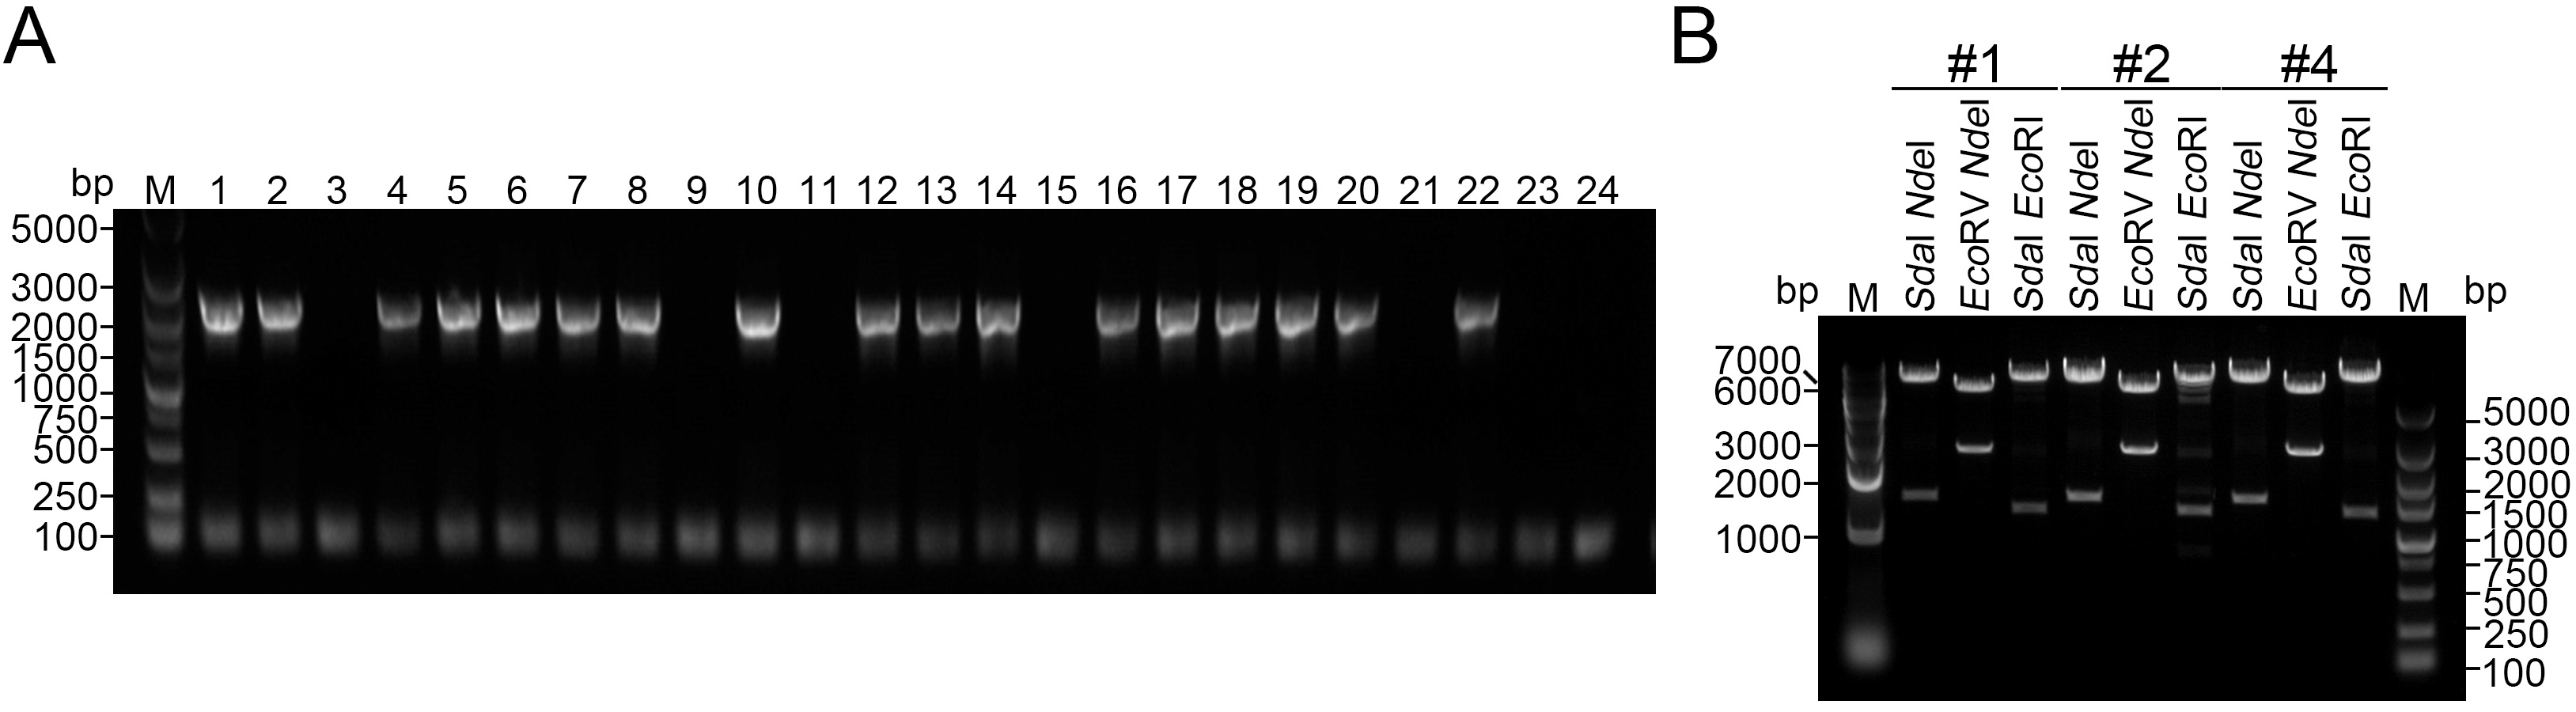
\includegraphics[width=\textwidth]{fig5-X.jpg}
%生成中英双语标题
{\setstretch{1.667}
\bicaption[fig:5.X]{图}{构建表达\ IFT52C::YFP::NLS\ 的载体\ pHK473。(A)\ 菌液\ PCR\ 筛选阳性克隆后的电泳结果。(B)\ 对图\ A\ 中的三个阳性克隆进行酶切验证。}{Figure}{The construction of pHK473 which can express IFT52C::YFP::NLS. (A) agarose gel electrophoresis of bacteria colony polymerase chain reaction product to screen positive clones. (B) Agarose gel electrophoresis of restriction enzyme digestion product of three representative positive clones.}
\par}
%结束图片浮动体环境
\end{figure}

IFT46-C1\ 是\ IFT46\ 的基体和纤毛定位序列。IFT52\ 结合并招募\ IFT46\ 至基体。根据已有的报道我们还知道衣藻中部分\ IFT46\ 与胞质囊泡关联并被转运到基体\ \citep{Wood2014}。然而,关于\ IFT46\ 基体定位的分子机制仍然存在两种可能性。一种是\ IFT52\ 和\ IFT46\ 独立定位基体并在基体中发生相互作用形成复合物。另一种是新合成的\ IFT46\ 和\ IFT52\ 在胞质中预组装成亚复合物并定位到基体。这两种途径的关键差别在于\ IFT46\ 和\ IFT52\ 发生相互作用形成复合物的位置。在第一种途径中,二者在基体发生相互作用。而在第二种途径中二者在胞质或\ TGN\ 中形成亚复合物。为了排除其中一种可能性,我们拟将\ IFT52C\ 异位表达在衣藻细胞核并检查\ IFT46\ 是否跟随\ IFT52C\ 富集在细胞核。

为了构建表达\ IFT52C::YFP::NLS\ 的\ pHK473,我们以\ pHK470\ 为模板,利用引物\ IFT52C-F\ 和\ IFT52C-R\ 进行扩增,扩增产物经纯化后利用\ In-Fusion\ 方法重组克隆。随机挑选二十四个单克隆进行进行菌液\ PCR\ 检测,电泳结果显示其中十七个克隆可扩增出目的条带
(图\ \ref{fig:5.X}A)。 从这十七个疑似阳性克隆中选择三个扩大培养,抽提质粒进行酶切验证。电泳结果显示\ \#1\ 号和\ \#4\ 号克隆为阳性(图\ \ref{fig:5.X}B)。选定酶切大小正确的克隆进行测序验证,没有发生错义突变的\ \#4\ 号克隆用于后续实验。

\subsection{融合\ NLS\ 标签的\ IFT52C\ 可将\ IFT46\ 招募到细胞核}
%开始图片浮动体环境,其中!表示取消严谨限制,h表示在此处插入,t表示在本页或下一页顶部插入
\begin{figure}[h!tbp]
%居中对齐
\centering
%设置图片搜索路径,每个路径用{}括起来
\graphicspath{{figures/}}
%插入图片并设置图片宽度为文本宽度减10mm
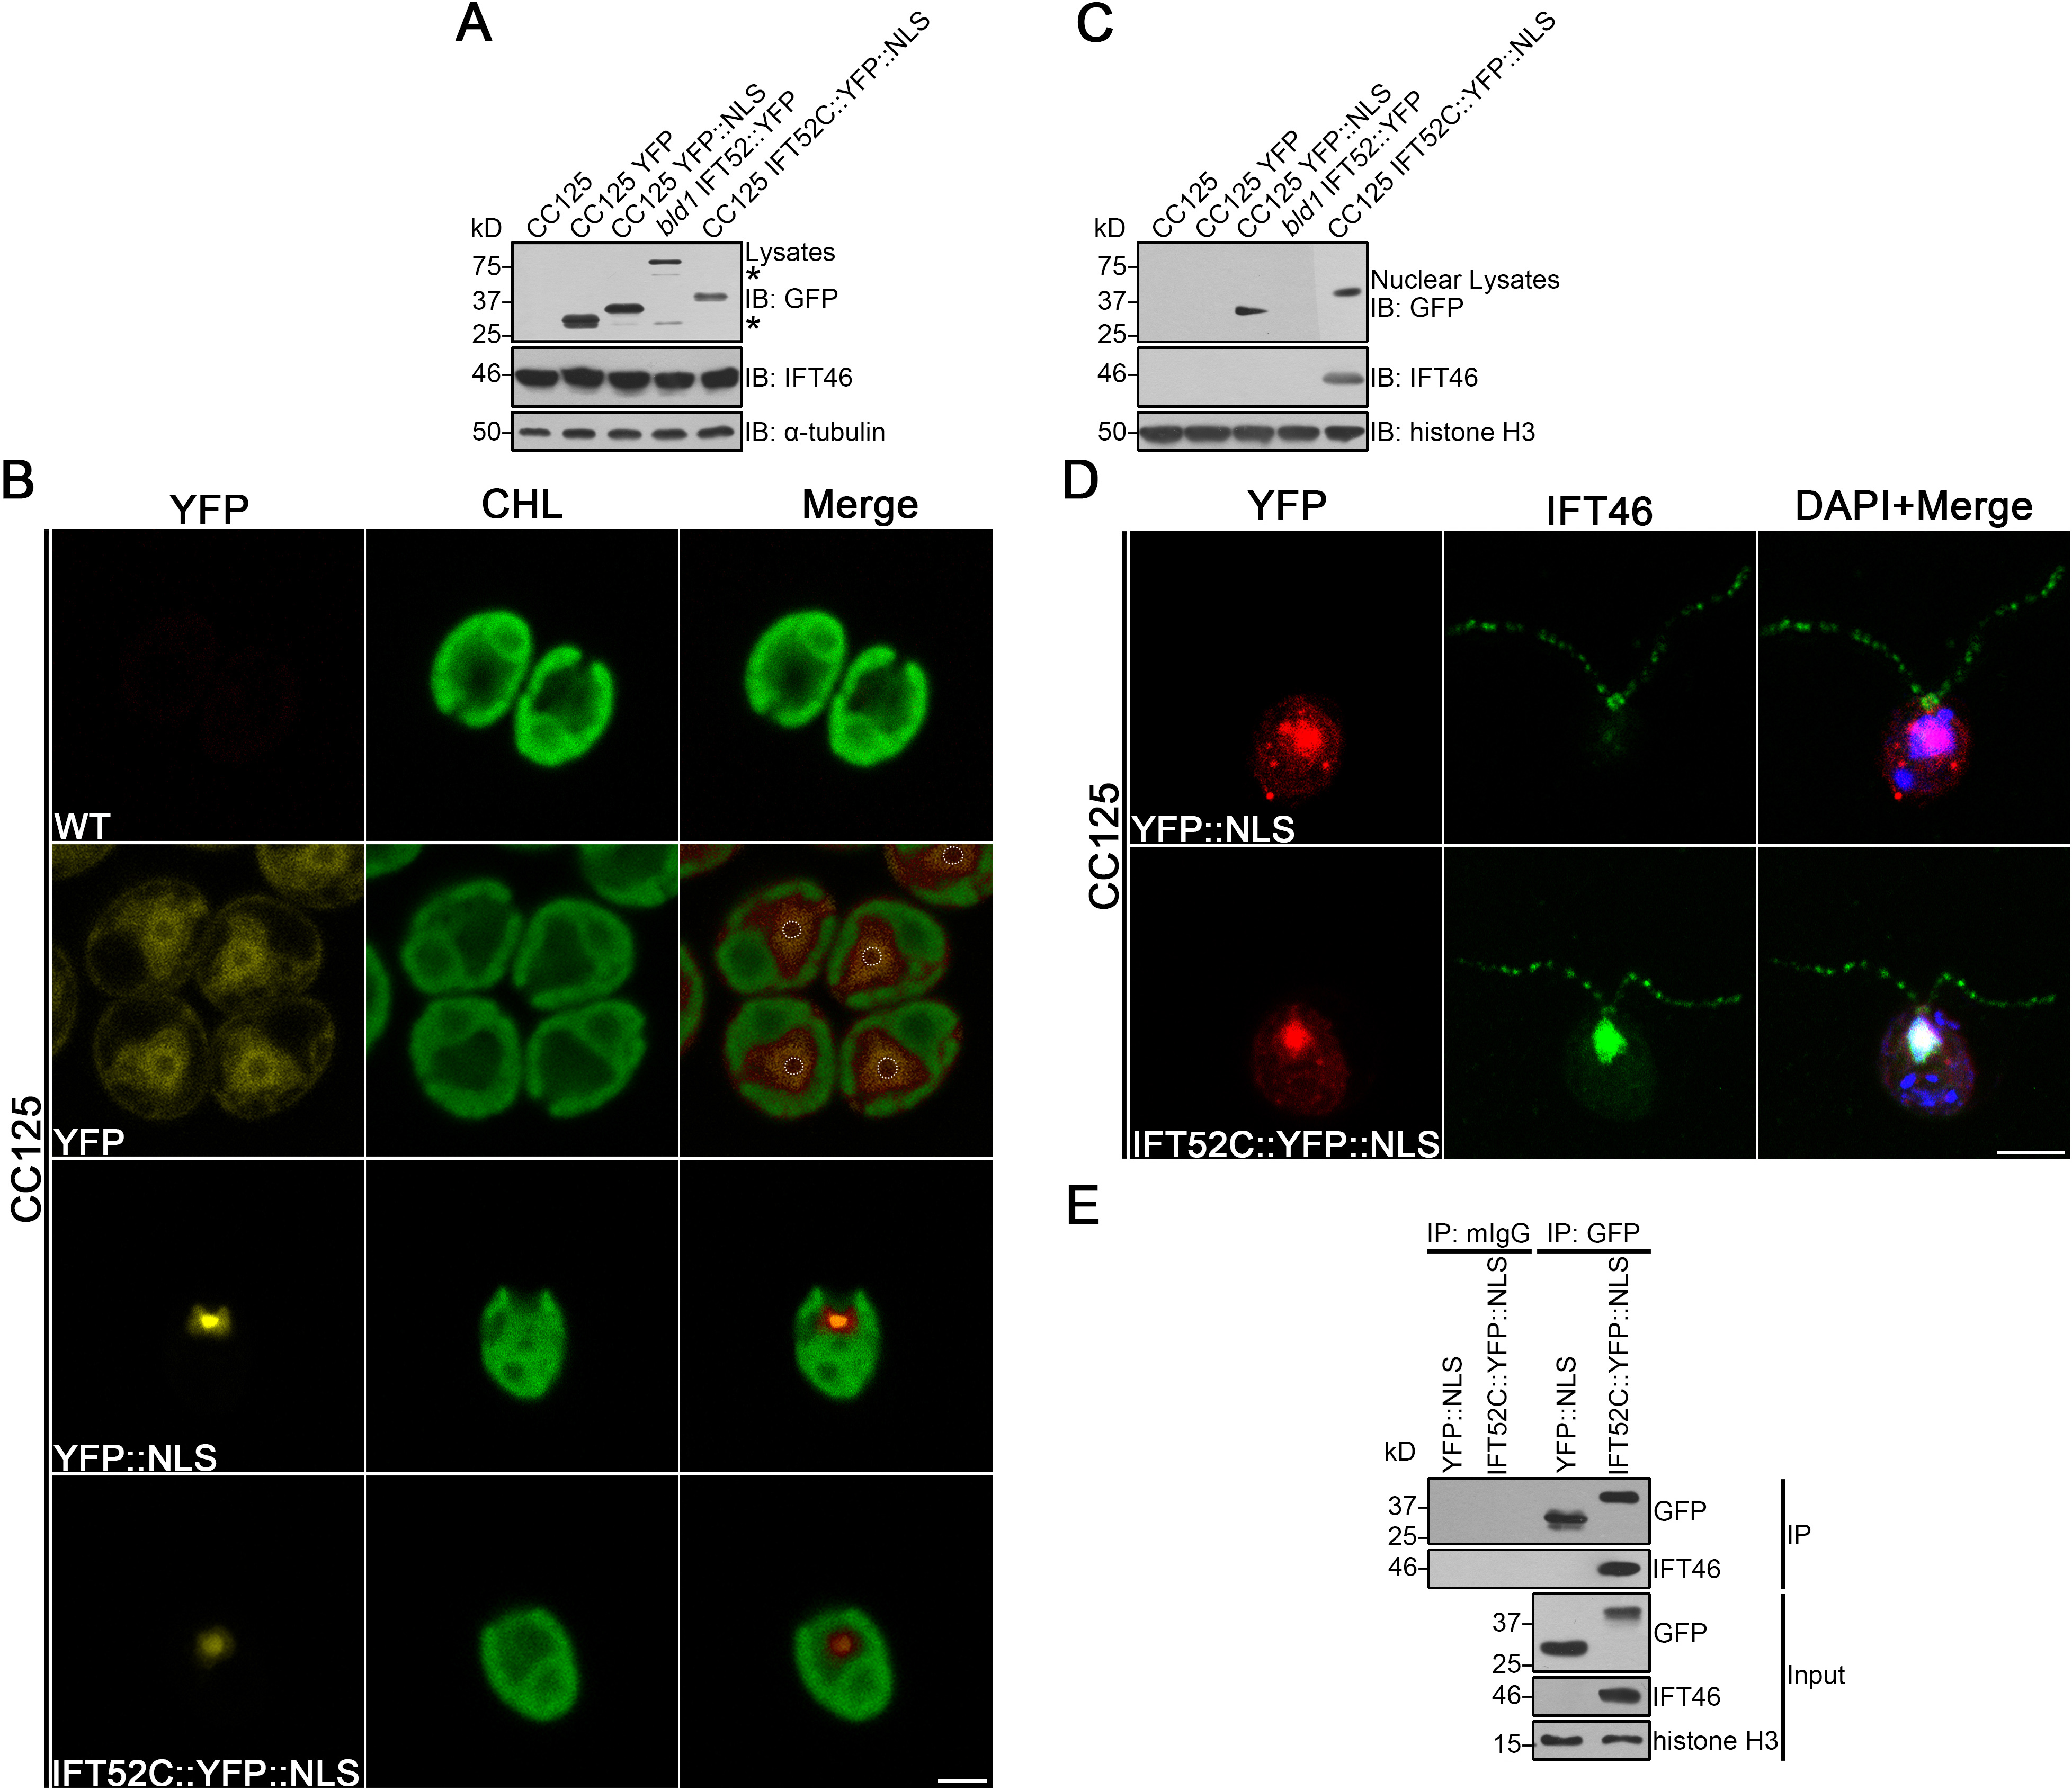
\includegraphics[width=\textwidth]{fig5-7.jpg}
%生成中英双语标题
{\setstretch{1.52}
\bicaption[fig:5.7]{图}{带\ NLS\ 标签的\ IFT52C\ 将\ IFT46\ 招募至细胞核。(A)\ 全细胞裂解物免疫印迹分析。(B)\ 表达\ YFP, YFP::NLS\ 和\ IFT52C::YFP::NLS\ 的\ CC-125\ 藻株的共聚焦成像分析。(C)\ CC-125, CC-125 \textit{YFP}, CC-125 \textit{YFP::NLS}, \textit{bld1} \textit{IFT52::YFP}\ 和\ CC-125 \textit{IFT52C::YFP::NLS}\ 核裂解物免疫印迹分析。(D)\ 藻株\ CC-125 \textit{YFP::NLS}\ 和\ CC-125 \textit{IFT52C::YFP::NLS}\ 免疫荧光成像。\textcolor{red}{红色}为\ YFP::NLS\ 或\ IFT52C::YFP::NLS,\textcolor{green}{绿色}为\ IFT46,\textcolor{blue}{蓝色}为标示细胞核的\ DAPI。(E)\ 使用抗\ GFP\  的抗体针对带\ YFP\ 标签的\ IFT52C::YFP::NLS\ 对\ CC-125 \textit{IFT52C::YFP::NLS}\ 细胞核裂解液进行免疫共沉淀分析。沉淀产物用图示抗体进行检测。}{Figure}{NLS-tagged IFT52C recruits IFT46 to nuclei. (A) Western blots of whole-cell lysates (\SI{5}{\ug} protein per lane) of indicated strains. (B) Live cell imaging of CC-125 and CC-125 expressing YFP, YFP::NLS and IFT52C::YFP::NLS. CHL, chlorophyll. (C) Western blots of nuclear lysates (\SI{2}{\ug} protein per lane) of indicated strains. (D) Immunofluorescence microscopy of CC-125 \textit{YFP::NLS} and CC-125 \textit{IFT52C::YFP::NLS} using anti-GFP antibody (red), anti-IFT46 antibody (green) and 4, 6-diamidino-2-phenylindole (DAPI, blue). (E) Anti-GFP antibody was used to immunoprecipiate IFT52C::YFP::NLS from the nuclei of CC-125 \textit{IFT52C::YFP::NLS}. mIgG, IgG; IB, immunoblot; Scale bars, \SI{5}{\um}.}
\par}
%结束图片浮动体环境
\end{figure}

在植物、动物和病毒中存在多种核定位信号\ \citep{Lange2007,Rasala2014,Kropat2005,Kalderon1984}。 然而关于核定位信号在衣藻中的报道并不多\ \citep{Rasala2014,Lauersen2015}。本实验室前期的工作表明\ 4xSV40 NLS\ 能够有效的将\ YFP\ 带至衣藻细胞核(Wan et al., unpublished data)。为简便起见,后文所称\ NLS\ 均指的是\ 4xSV40 NLS。根据已有报道,IFT52\ 通过其\ C\ 端与\ IFT46\ 相互作用\
\citep{Taschner2016a,Lucker2005,Lucker2010,Taschner2011,Taschner2014,Katoh2016}。此外,在\ MDCK\ 细胞中过表达\ MmIFT52C\ 对初级纤毛的形成具有极强的显性负效应\ \citep{Taschner2014}。这可能是由其他\ IFT-B\ 蛋白的错误定位导致的\
\citep{Taschner2014}。以上事实表明将\ NLS\ 融合在\ IFT52C\ 上来研究\ IFT\ 蛋白的定位非常合适。

在野生型\ CC-125\ 细胞中,我们使用抗\ GFP\ 的抗体通过免疫印迹筛选出表达\ IFT52C::YFP::NLS\ 的阳性克隆(图\ \ref{fig:5.7}A)。通过共聚焦显微成像我们发现\ IFT52C::YFP::NLS\ 能够有效定位到衣藻细胞核(图\ \ref{fig:5.7}B)。对\ CC-125 \textit{IFT52C::YFP::NLS}\ 的细胞核的裂解液进行免疫印迹分析也证实\ IFT52C::YFP::NLS\ 确实成功在核内表达
(图\ \ref{fig:5.7}C)。与此同时,我们在\ CC-125 \textit{IFT52C::YFP::NLS}\ 的细胞核中也检测到了\ IFT46 (图\ \ref{fig:5.7}C)。免疫荧光实验的结果显示\ IFT46\ 除定位在基体和鞭毛外,在基体下方还与\ DAPI\ 共定位(图\ \ref{fig:5.7}D)。这表明\ IFT46\ 跟随\ IFT52C\ 进入了细胞核。使用抗\ GFP\ 的抗体对\ CC-125 \textit{IFT52C::YFP::NLS}\ 的核裂解液进行免疫共沉淀,结果显示\ IFT52C\ 与\ IFT46\ 均富集在沉淀物中(图\ \ref{fig:5.7}E)。这些数据表明\ IFT46\ 能够被融合了\ NLS\ 标签的\ IFT52C\ 招募到细胞核。这意味着二者在细胞质中已经预组装成亚复合物。

\section{讨论}
%开始图片浮动体环境,其中!表示取消严谨限制,h表示在此处插入,t表示在本页或下一页顶部插入
\begin{figure}[htbp]
%居中对齐
\centering
%设置图片搜索路径,每个路径用{}括起来
\graphicspath{{figures/}}
%插入图片并设置图片宽度为文本宽度减10mm
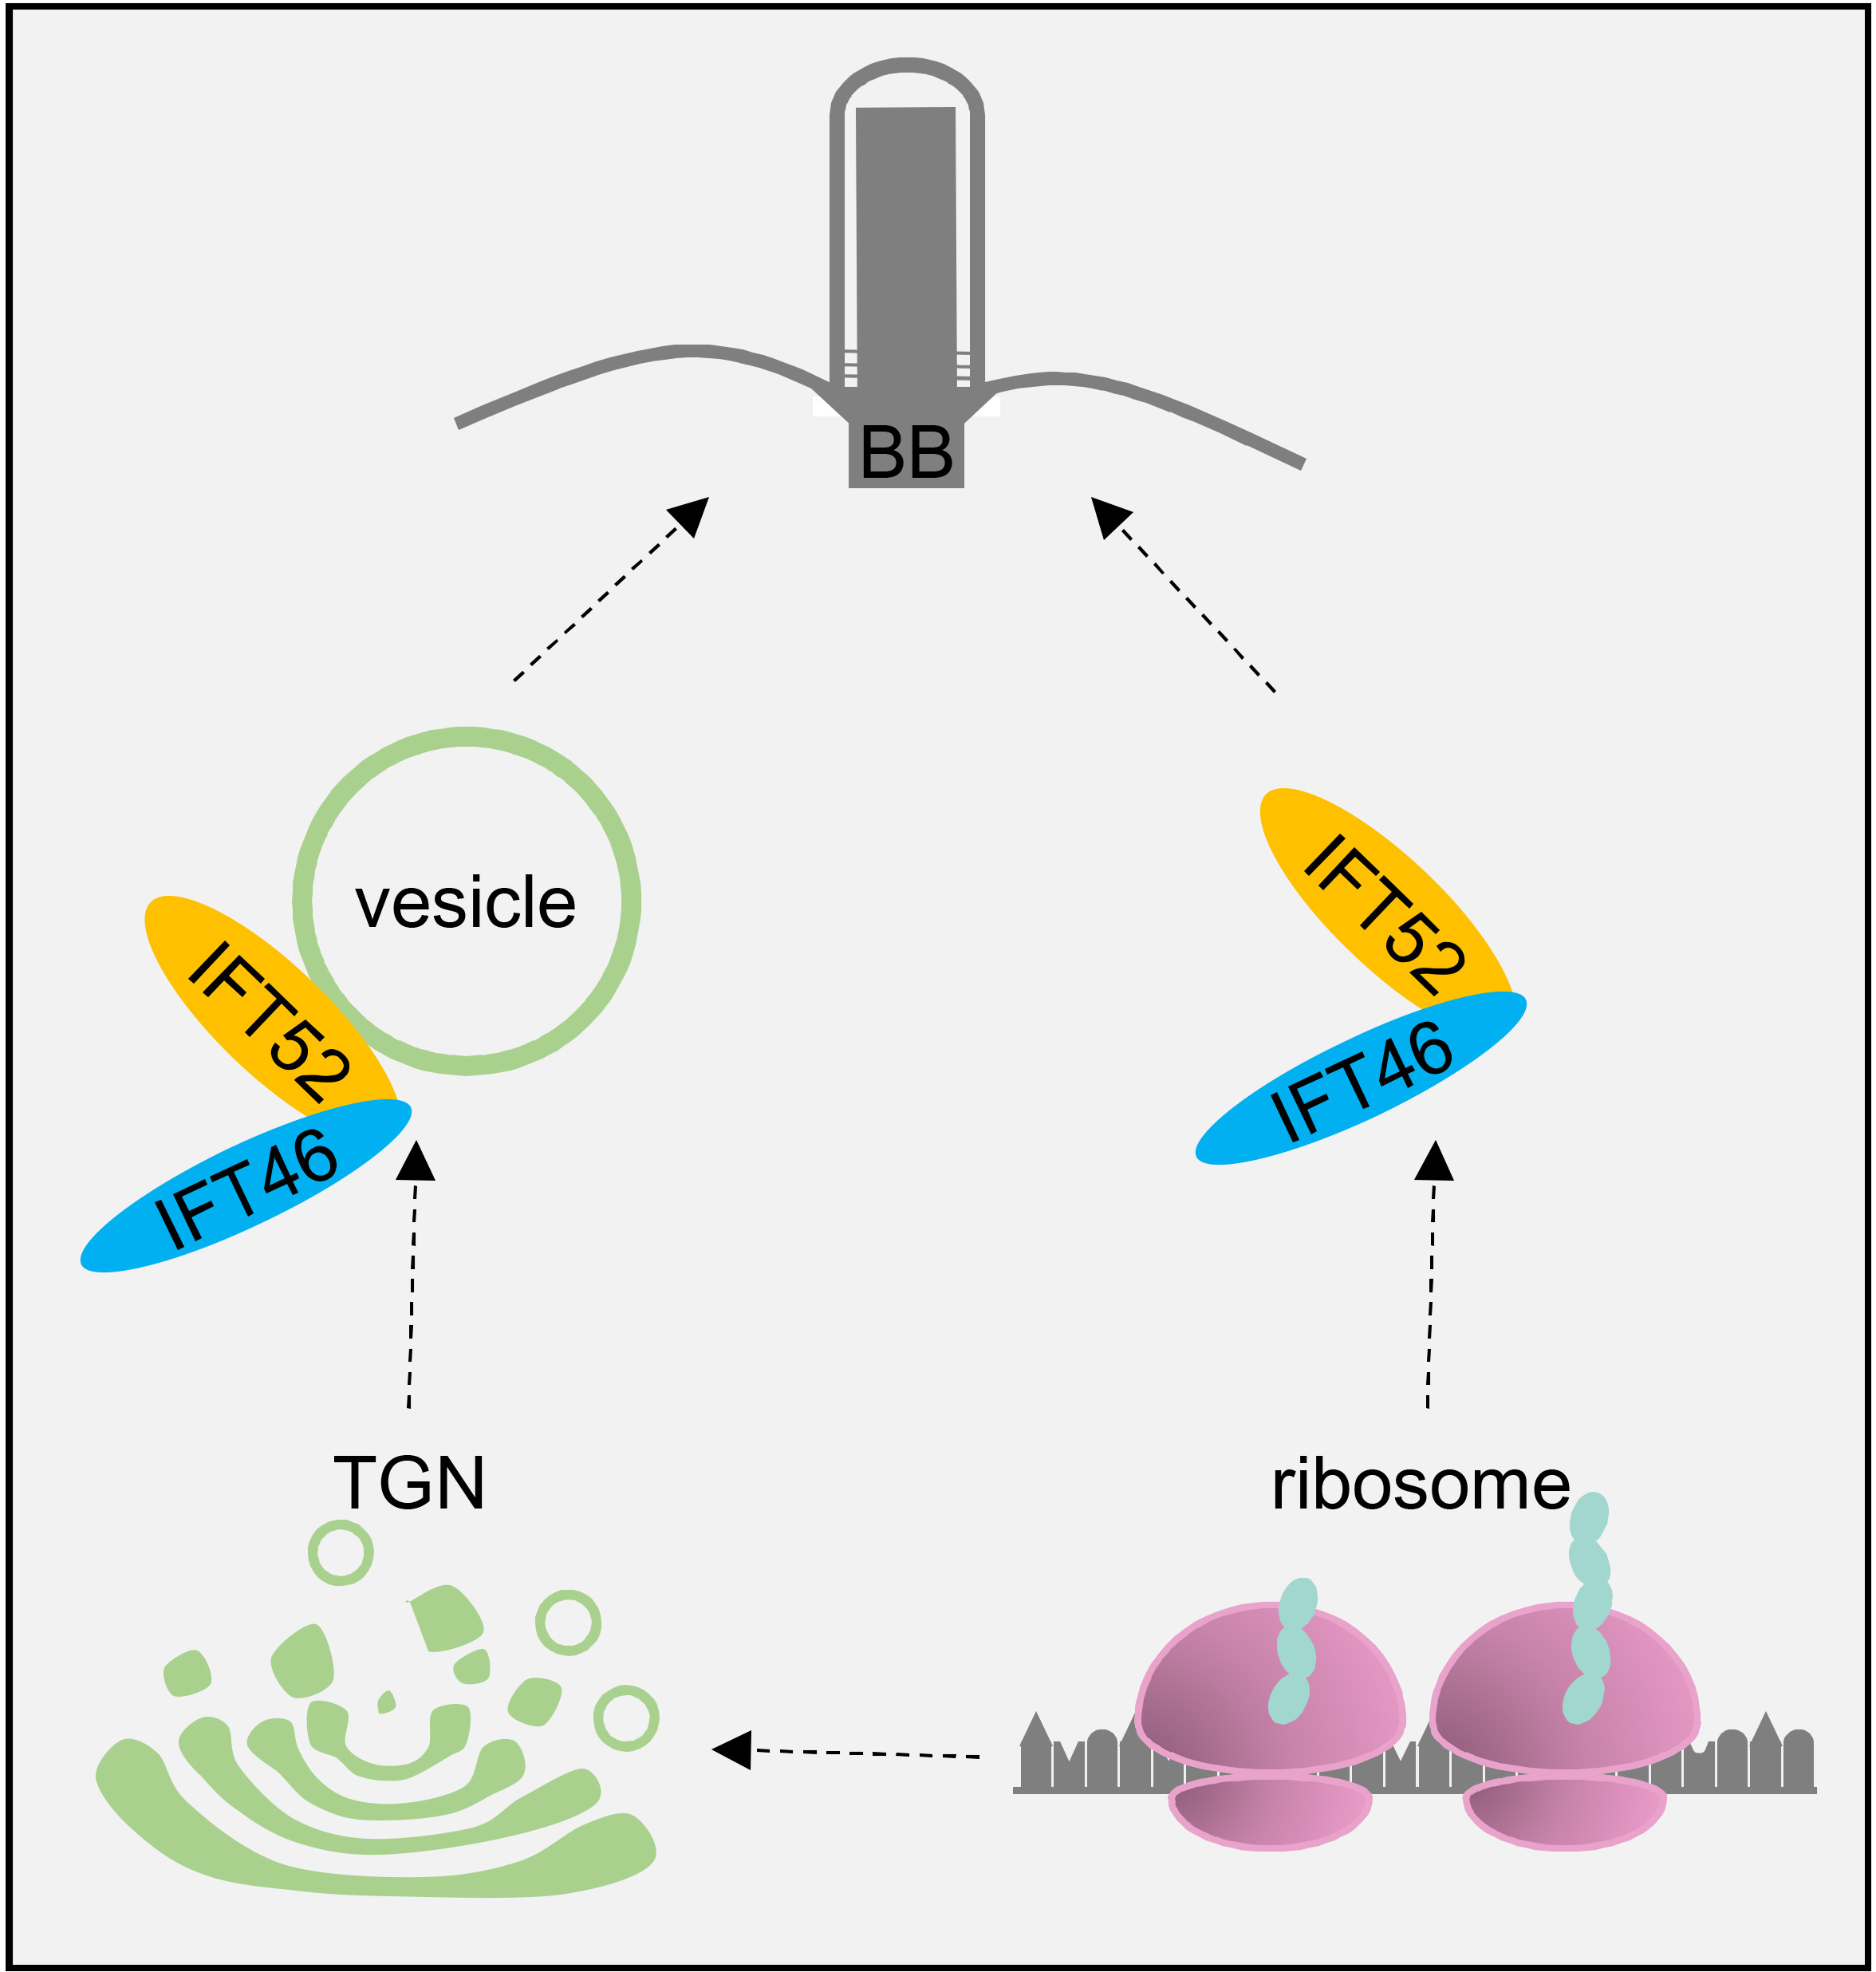
\includegraphics[width=\textwidth-80mm]{fig5-8.jpg}
%生成中英双语标题
{\setstretch{1.667}
\bicaption[fig:5.8]{图}{IFT46\ 基体定位的模型。核糖体上合成的\ IFT46\ 和\ IFT52\ 在胞质或高尔基体上预组装成亚复合物并经过囊泡或非囊泡介导的途径定位到基体。TGN\ 为反式高尔基体网络,BB\ 为基体。}{Figure}{Model for basal body localization of IFT46. Preassembled IFT52/46 subcomplex is targeted to basal body region through the vesicle-mediated or non-vesicle-mediated ways. TGN, trans-Golgi network; BB, basal body.}
\par}
%结束图片浮动体环境
\end{figure}

IFT46\ 的\ C\ 端是\ IFT46\ 的基体和纤毛定位序列\ \citep{Lv2017}。IFT52\ 结合并招募\ IFT46\ 至基体\ \citep{Lv2017}。同时\ IFT46\ 能够被含\ NLS\ 标签的\ IFT52C\ 招募到细胞核\ \citep{Lv2017}。这表明\ IFT46\ 和\ IFT52\ 是在胞质或\ TGN\ 中预组装而非在基体中才组装\ \citep{Lv2017}。在衣藻鞭毛再生过程中,IFT46\ 出现在来自\ TGN\ 的囊泡上\ \citep{Wood2014}。因而有可能\ IFT46\ 和\ IFT52\ 是在\ TGN\ 中预组装并通过囊泡介导的途径定位到基体(图\ \ref{fig:5.8})。然而,在\ IFT\ 蛋白中仅\ IFT20\ 曾被观察到定位在高尔基体,大部分\ IFT\ 蛋白均与膜没有关联\
\citep{Richey2012,Follit2006}。 因此我们无法排除这样一种可能性,即预组装的\ IFT46\ 和\ IFT52\ 通过非囊泡介导的途径定位到基体(图\ \ref{fig:5.8})。

与\ Lucker\ 和\ Richey\ 等人提出的关于\ IFT\ 复合物\ B\ 的组装模型相比,三者均认为\ IFT\ 复合物\ B\ 中的亚基预组装成亚复合物,这些亚复合物再组装成完整的复合物\ B\ \citep{Lucker2010,Richey2012,Lv2017}。 不同之处在于我们提供了有力的证据显示\ IFT52\ 作用在\ IFT46\ 的上游,发挥类似“种子”的作用\ \citep{Lv2017}。除了能够结合并招募\ IFT46,我们认为\ IFT52\ 很可能还招募了其他亚基。然而受限于相应的抗体和突变体,这种假设需要通过其他途径进行验证。此外,三个模型中关于复合物组装的位置有差异。Lucker\ 等人的模型未明确指出组装发生的地点\ \citep{Lucker2010}。这可能是由于他们的大部分结果均通过生化方法获得,缺少体内实验的验证。Richey\ 等人的模型则认为\ IFT\ 复合物\ B\ 的核心复合物可能在基体近端组装然后转移到过渡纤维\ \citep{Richey2012}。这种转变过程需要\ IFT88\ 和\ IFT\ 复合物\ B\ 外周亚基的参与\ \citep{Richey2012}。这一模型虽然信息完善,但大多属于猜测,可靠性有待进一步证实。根据我们的实验结果,我们认为\ IFT52\ 和\ IFT46\ 在胞质中预先组装成亚复合物然后再定位到基体(图\ \ref{fig:5.8})。当然,这里还有很多问题有待解决。比如还有哪些亚基参与了预组装,亚复合物定位到基体的什么部位等。一种可行的研究策略是异位表达\ IFT52,然后通过亲和纯化分离特定细胞器并通过质谱鉴定哪些蛋白跟随\ IFT52\ 发生了转位。

前面我们发现\ IFT46-C1\ 是\ IFT46\ 的基体定位序列。这里我们检测到\ IFT46-C1\ 直接与\ IFT52\ 相互作用(图\ \ref{fig:5.6})。通过突变\ IFT46-C1\ 上的关键残基来破坏\ IFT46-C1\ 与\ IFT52\ 之间的相互作用可阻断\ IFT46-C1\ 的基体定位(图\ \ref{fig:5.6})。这表明\ IFT52\ 直接介导了\ IFT46\ 的基体定位。然而,IFT46\ 的相互作用对象仍然是一个\ IFT\ 蛋白,IFT52。 这使得\ IFT46-C1\ 有别于其他的经典定位序列\
\citep{Malicki2014,Bhogaraju2013,McIntyre2015,Dishinger2010,Berbari2008,Hurd2011,Santos2014}。 在接下来的工作中我们需要在\ IFT52\ 或其他上游\ IFT\ 蛋白中鉴定到\ IFT\ 蛋白通用的定位序列。

\section{小结}
通过在\ IFT\ 相关蛋白的缺失突变体中表达\ IFT46\ 或\ IFT46-C1,我们发现\ IFT46\ 的基体定位不依赖\ IFT122、IFT88、IFT81、FLA10\ 或\ DHC1b,但是依赖\ IFT52。同时\ IFT52\ 的基体定位并不依赖\ IFT46。 这说明\ IFT52\ 作用在\ IFT46\ 的上游。进一步研究发现\ IFT52\ 能够结合并招募\ IFT46\ 至基体。通过在细胞核中表达\ IFT52C,我们成功将\ IFT46\ 招募到细胞核。这些结果表明\ IFT46\ 和\ IFT52\ 在细胞质或\ TGN\ 中预组装成亚复合物然后定位到基体(图\ \ref{fig:5.8})。 